 % DOCUMENTO PRINCIPAL

% Este es el fichero principal de este repositorio. No se recomienda editarlo.
% Modifica las plantillas incluidas en los directorios:
% - secciones
% - tablas
% - algoritmos

\documentclass[final,a4paper,12pt,twoside]{class_diss}

\usepackage[full]{textcomp}
\usepackage{graphicx}
\usepackage{amsmath}
\usepackage{amsxtra}
\usepackage{amssymb}
\usepackage{amsthm}
\usepackage{latexsym}
\usepackage{setspace}
\usepackage[margin=3cm]{geometry}
\usepackage[titles]{tocloft}
\usepackage{latexsym}
\usepackage{fancyhdr}
\usepackage{emptypage}
\usepackage[svgnames,dvipsnames,usenames,table,xcdraw]{xcolor}
\usepackage{tikz}
\usepackage[toc,acronym,nonumberlist,xindy={language=spanish-traditional}]{glossaries}
\usepackage[scaled]{helvet}
\usepackage[utf8]{inputenc}
\usepackage[T1]{fontenc}
\usepackage[spanish,es-tabla]{babel}
\usepackage[explicit]{titlesec}
\usepackage{newtxtext}
\usepackage{newtxmath}
\usepackage{stmaryrd}
\usepackage{bbold}
\usepackage[ruled,vlined]{algorithm2e}
\usepackage{algorithmic}
\usepackage{float}
\usepackage{url}
\usepackage{xspace}
\usepackage{booktabs}
\usepackage{multirow}
\usepackage{enumitem}
\usepackage{rotating}
\usepackage{pdflscape}
\usepackage{listings}
\usepackage{placeins}
\usepackage{flafter}

\theoremstyle{definition}
\newtheorem{definition}{Teorema}[section]
\theoremstyle{remark}
\newtheorem*{remark}{Remark}
\DeclareMathOperator*{\argmax}{arg\,max}
\DeclareMathOperator*{\argmin}{arg\,min}
\definecolor{VIU}{RGB}{240, 90, 15}
\definecolor{DESTACADO}{RGB}{130, 34, 145}
\definecolor{CITA}{RGB}{0, 123, 194}
\definecolor{GRAY}{RGB}{100, 100, 100}

%\renewcommand{\algorithmcfname}{Algoritmo}
\renewcommand{\acronymname}{Lista de Acr\'onimos}
\addto\captionsspanish{
    \renewcommand*{\acronymname}{Lista de Acr\'onimos}
}
\newcommand{\inhib}{\relbar\mapsfromchar}
\newcommand{\destacado}[1]{\color{DESTACADO}\textbf{#1}\color{black}\xspace}

\usetikzlibrary{shapes}
\newcommand*\circled[1]{\tikz[baseline=(char.base)]{
    \node[shape=circle,fill=GRAY!90,inner sep=1pt,minimum size=1cm] (char) {\textcolor{white}{\small\textbf{#1}}};}
}

\pagestyle{fancy}
\fancyhf{}
\fancyhead[LO]{}
\fancyhead[RE]{}
\fancyfoot[C]{}
\renewcommand{\headrulewidth}{0pt}

\fancypagestyle{plain}{
  \fancyhf{}
  \fancyfoot[C]{\circled{\thepage}}
  \renewcommand{\headrulewidth}{0pt}
}

\colorlet{chapnumcolor}{VIU}

\newcommand*{\chapnumfont}{%
  \usefont{T1}{jkp}{b}{n}%
  \fontsize{70}{90}%
  \selectfont%
}

\newcommand*{\chaptitlefont}{%
  \usefont{T1}{qhv}{b}{n}%
  \fontsize{22}{26}%
  \selectfont%
}

\titleformat{name=\chapter}
{\normalfont\huge\bfseries}
{\rlap{\parbox{\textwidth}{\filleft\chapnumfont\color{chapnumcolor}\thechapter}}}
{0pt}
{\rlap{\parbox{0.7\textwidth}{\filright\chaptitlefont #1}}}

\makeglossaries
% GLOSARIO

% Si quieres incluir un glosario y una lista de abreviaturas en tu Trabajo Fin de Máster,
% sigue las instrucciones indicadas en la siguiente URL:
% https://www.overleaf.com/learn/latex/glossaries

\newacronym{acr_nlp}{NLP}{Procesamiento del Lenguaje Natural o \textit{Natural Language Processing}}
\newacronym{acr_squad}{SQuAD}{The Stanford Question Answering Dataset}
\newacronym{acr_ml}{ML}{Aprendizaje Automático o \textit{Machine Learning}}
\newacronym{acr_dl}{DL}{Aprendizaje Profundo o \textit{Deep Learning}}
\newacronym{acr_rnn}{RNN}{Redes Neuronales Recurrentes o \textit{Recurrent Neural Networks}}
\newacronym{acr_cnn}{CNN}{Redes Neuronales Convolucionales o \textit{Convolutional Neural Networks}}
\newacronym{acr_ffnn}{FFNN}{Redes Neuronales Prealimentadas o \textit{Feed Forward Neural Networks}}
\newacronym{acr_dnn}{DNN}{Redes Neuronales Profundas o \textit{Deep Neural Networks}}
\newacronym{acr_lstm}{LSTM}{Redes de Gran Memoria a Corto Plazo o \textit{Long Short-Term Memory}}
\newacronym{acr_tpu}{TPU}{Unidad de Procesamiento Tensorial o \textit{Tensor Processing Unit}}
\newacronym{acr_gpu}{GPU}{Unidad de Procesamiento Gráfico o \textit{Graphic Processing Unit}}
\newacronym{acr_html}{HTML}{Lenguaje de Marcas de Hipertexto o \textit{HyperText Markup Language}}

\newglossaryentry{gls_wordembeddings}
{
        name=Word Embeddings,
        text=\textit{word embeddings},
        description={es una técnica del procesamiento del lenguaje natural que consiste, básicamente, en asignar un vector a cada palabra. Este vector guarda información semántica, lo que permite que pueda ser asociado o disociado a otros vectores (palabras) según distintos contextos gramaticales}
}

\newglossaryentry{gls_transformer}
{
        name=Transformer,
        text=transformer,
        description={son una clase reciente de redes neuronales para datos de tipo secuenciales, basadas en la autoatención, que han demostrado estar bien adaptadas al texto y actualmente están impulsando importantes avances en el procesamiento del lenguaje natural}
}

\newglossaryentry{gls_softmax}
{
        name=Softmax,
        name=\textit{softmax},
        description={La función Softmax es una función de activación que transforma las salidas a una representación en forma de probabilidades, de tal manera que el sumatorio de todas las probabilidades de las salidas de 1. Devuelve la distribución de probabilidad de cada una de las clases soportadas en el modelo}
}

\newglossaryentry{gls_json}
{
        name={Archivo JSON},
        text={\textit{archivo .json}},
        description={Notación de Objeto Javascript o JavaScript Object Notation (JSON) es un formato de archivo sencillo para el intercambio de información. El formato JSON permite representar estructuras de datos (arrays) y objetos (arrays asociativos) en forma de texto}
}

\newglossaryentry{gls_tfidf}
{
        name={TF-IDF},
        description={TF-IDF (del inglés Term frequency – Inverse document frequency), frecuencia de término – frecuencia inversa de documento, es una medida numérica que expresa cuán relevante es una palabra para un documento en una colección, calculada a través de la frecuencia de ocurrencia del término en la colección de documentos}
}

\newglossaryentry{gls_computer_vision}
{
        name={Computer Vision},
        text={\textit{computer vision}},
        description={Disciplina científica que incluye métodos para adquirir, procesar, analizar y comprender las imágenes del mundo real con el fin de producir información numérica o simbólica para que puedan ser tratados por un ordenador.}
}



\bibliographystyle{apa}

\usepackage[authoryear,sort&compress]{natbib}
\usepackage{hypernat}
\setcitestyle{authoryear}

\usepackage[pdftex,plainpages=false,pdfpagelabels]{hyperref}

\hypersetup{
    linktocpage=true,
    colorlinks=true,
    %bookmarks=true,
    citecolor=CITA,
    urlcolor=CITA,
    linkcolor=CITA,
    citebordercolor={1 0 0},
    urlbordercolor={1 0 0},
    linkbordercolor={.7 .8 .8},
    breaklinks=true,
    %pdfpagelabels=true,
    }

\setcounter{secnumdepth}{3}
\onehalfspacing
\renewcommand\familydefault{\sfdefault}

\begin{document}

\begin{figure}[H]
	\begin{center}
		
\includegraphics[scale=0.25]{figuras/logo-viu.png}
	\end{center}
\end{figure}

\begin{center}
	\begin{bf}
		{\large MÁSTER UNIVERSITARIO\\EN INTELIGENCIA ARTIFICIAL}\\
	\end{bf}
	\vspace*{5cm}
	
	\begin{bf}
		%{\large Desarrollo de aplicaciones de NLP usando el nuevo modelo de Google, Bidirectional Encoder Representations from Transformer (BERT)}\\
		{\large Implementación y evaluación de aplicaciones usando BERT, para los problemas de análisis de sentimiento y respuesta a preguntas.} \\
	\end{bf}
	
	{\large \textit{Curso académico 2021-22 - Matrícula abril 2021}}\\
	{\large \textit{Tercera convocatoria: mayo 2022}}\\
	
	\vspace{5 cm}
\end{center}

%\begin{flushleft}
%	
%	{\large \textbf{Dirigido por:} Díaz Pinto, Andrés Yesid}\\
%	\textbf{e-mail:} \href{andresyesid.diaz@campusviu.es}{andresyesid.diaz@campusviu.es}\\
%	
%\end{flushleft}

%\vspace*{1.3cm}
\begin{flushright}
	Por el alumno
	%{\large 
	\textbf{Izaguirre Viera, Luis Arturo}
	%}
	\\
	%\textbf{email:} 
	
	\textbf{DNI (Chile):} 24.767.484-5\\
	\href{lsizaguirre@gmail.com}{lsizaguirre@gmail.com}\\
	\vspace*{1cm}
	
	Dirigido por
	%{\large 
	\textbf{Díaz Pinto, Andrés}
	%}
	\\
	%\textbf{email:} 
	\href{andresyesid.diaz@campusviu.es}{andresyesid.diaz@campusviu.es}\\
\end{flushright}

\newpage



\cleardoublepage

% Frase favorita
\null\vspace{\stretch{2}}
{
	\hfill \begin{minipage}{8cm}
		\textsl{
			\begin{flushright}
				``It’s not artificial intelligence I’m worried about,\\ it’s human stupidity!''
			\end{flushright}
		}
		
		% Autor
		\begin{flushright}
			Neil Jacobstein
		\end{flushright}
	\end{minipage}
}
\vspace{\stretch{1}}

\pagenumbering{gobble}
\begin{onehalfspace}
% AGRADECIMIENTOS

\cleardoublepage

\normalfont{\huge{\bfseries{Agradecimientos}}}
\vspace{15ex}

A mis padres, por su inconmesurable amor, por siempre guiarme, por inspirarme a seguir sus pasos y ser cada día mejor.
\medskip
\medskip

A Nancy Victoria, quien ha sabido enseñarme a luchar por mis metas y a nunca rendirme. Gracias por tu apoyo incondicional.
\medskip
\medskip

A todo el cuerpo docente de la Universidad Internacional de Valencia por su dedicación y enseñanza. En especial al director de este trabajo, Andrés Díaz Pinto.
\medskip
\end{onehalfspace}
\cleardoublepage

\newpage
\pagenumbering{roman}
\setcounter{page}{1}

\pagestyle{fancy}
\fancyhf{}
\fancyhead[LO]{\leftmark}
\fancyhead[RE]{\rightmark}
\fancyfoot[C]{\circled{\thepage}}
\renewcommand{\headrulewidth}{0.4pt}
\setlength{\headheight}{14.49998pt}

\pdfbookmark[0]{\contentsname}{contents}

\renewcommand{\cftchapleader}{\cftdotfill{\cftdotsep}}
\renewcommand{\cftchapfont}{\mdseries}
\renewcommand{\cftchappagefont}{\mdseries}

\tableofcontents
\listoffigures
\listoftables

%\renewcommand{\listalgorithmcfname}{Índice de algoritmos}
%\listofalgorithms
%\addcontentsline{toc}{chapter}{Índice de algoritmos}

\newpage
\pagenumbering{arabic}
\setcounter{page}{1}

\setlength{\parskip}{1mm}

\begin{onehalfspace}
\cleardoublepage

\chapter*{Resumen}
\label{chpater-resumen}
\addcontentsline{toc}{chapter}{Resumen}

\textbf{BERT}, siglas para \textit{\textbf{B}idirectional \textbf{E}ncoder \textbf{R}epresentations from \textbf{T}ransformers} es un modelo de lenguaje preentrenado basado en la arquitectura de transformers que desde su aparición en octubre del 2018 ha avanzado en de forma acelerada en el estado del arte de diversas tareas comprendidas en el campo del procesamiento del lenguaje natural, como el resumen de textos, clasificación, similaridad semántica, entre otras.

El objetivo de este trabajo de investigación es evaluar el uso, la facilidad de implementación y el rendimiento que puede obtener este modelo en la solución de tareas para las que en un principio no fue entrenado.

Se eligió trabajar con dos tareas, la primera de ellas fue un problema de clasificación a través del análisis de sentimiento sobre un conjunto de datos que contiene reseñas de películas y la segunda un problema de comprensión lectora donde se intenta identificar una respuesta dada una pregunta y un contexto. Para resolver ambos problemas se realizó un proceso de ajuste o fine-tunning sobre el modelo base de BERT. 

Los resultados mostraron además de la facilidad de implementación, un excelente rendimiento al compararlo con los modelos que definen el estado del arte para cada una de estas tareas. Con un ligero proceso de ajuste se logró tener para el primer problema una precisión cercana al 92\% y para el problema de preguntas y respuestas un score F1 cercano al 77\%.

Los resultados sugieren que BERT es un excelente punto de partida para la construcción de soluciones a distintos problemas en el campo del procesamiento de lenguaje natural. 
% INTRODUCCIÓN

\cleardoublepage

\chapter{Introducción}
\label{chapter-introduccion}

\section{Procesamiento Natural del Lenguaje}
\label{section-procesamiento-natural-lenguaje}

Los últimos años hemos sido testigos del auge de la inteligencia artificial y del impacto que esta ha generado en distintos aspectos de nuestras vidas, convirtiéndose en una tecnología que ha cambiado la forma en la que interactuamos y vivimos. Hemos presenciado sorprendentes avances de la inteligencia artificial en distintos ámbitos y la evolución que ha tenido en la resolución de muchas tareas específicas, logrando en varias de ellas superar las capacidades cognitivas propias de los seres humanos. 

El \acrlong{acr_nlp} (\acrshort{acr_nlp}, por sus siglas en inglés) es una rama de la inteligencia artificial que habilita a las computadoras a comprender, entender y procesar el lenguaje humano. El \acrshort{acr_nlp} provee de un conjunto de técnicas y metodologías para analizar, interpretar y darle significado al lenguaje y de este modo, poder generar conocimiento a partir de este. 

El \acrshort{acr_nlp} se ha convertido en una de las tareas más complejas a resolver en la búsqueda de recrear las capacidades cognitivas propias de los seres humanos a través de las máquinas. Y es que, sin lugar a duda, el lenguaje humano es un proceso bastante complejo que ha sido el resultado de la propia evolución a lo largo de miles de años y sustentado por un motor biológico con más de cien mil millones de neuronas que interactúan entre sí. 

Para hacerlo aún más complejo, nuestro lenguaje está lleno de ambigüedades, de palabras con distintas acepciones, giros y diversos significados según el contexto y además elementos que aún son de difícil comprensión como la ironía o el sarcasmo. Esto hace que el procesamiento de lenguaje natural haya sido una de las tareas más difíciles de dominar en el mundo de la inteligencia artificial.
\medskip

\section{El aprendizaje automático y el NLP}
\label{section-antes-de-las-redes-neuronales}

En este camino del entendimiento y comprensión del lenguaje humano por las maquinas, se han explorado distintas soluciones desde algoritmos o arquitecturas basadas en reglas donde se intenta modelar instrucción a instrucción y a través de reglas complejas, hasta soluciones donde dejamos que algoritmos puedan inferir estas reglas a través del \acrlong{acr_ml} (\acrshort{acr_ml}, por sus siglas en inglés). 

El \textit{machine learning} a pesar de ser una disciplina con muchos años de investigación, ha ganado una relevancia considerable en los últimos años debido al aumento cada vez mayor de la capacidad de cómputo y con ello la habilidad de poder procesar grandes cantidades de datos. Esto ha posibilitado el desarrollo acelerado del \textit{machine learning} y los modelos de \acrlong{acr_dl} (\acrshort{acr_dl}, por sus siglas en inglés). Las redes neuronales artificiales ocupan una posición muy prometedora en el área del \textit{machine learning} y han transformado la forma en que se desarrollan las aplicaciones de \acrshort{acr_nlp}. 

Para este tipo de problemas donde el dato de entrada es un texto de naturaleza secuencial, se han explorado distintas arquitecturas que van desde las redes neuronales recurrentes (ver sección \ref{section-rnn}), pasando por las redes \textit{long short-term memory} (ver sección \ref{section-lstm}), hasta las poderosas redes basadas en la novedosa arquitectura de \Gls{gls_transformer}, concepto sobre el que se profundizará en la sección \ref{subsection-atencion-transformer}.

\subsection{Redes Neuronales Recurrentes (RNN)}
\label{section-rnn}

Las \acrlong{acr_rnn} (\acrshort{acr_rnn}, por sus siglas en inglés), son un tipo de redes que tienen un excelente desempeño para el análisis de datos que tienen una naturaleza secuencial, es decir, datos donde el orden tiene importancia relevante. Es por ello, que generalmente es empleada en los problemas de procesamiento de audio, vídeo o texto. La idea es que los datos de entrada tengan una cierta secuencia adjunta como en los textos donde la secuencia de palabras genera un contexto que agrega significado a la oración. 

Como es explicado por \cite{torres2019deep}, las redes neuronales recurrentes fueron concebidas en la década de 1980. Pero estas redes fueron en un principio difíciles de entrenar por sus requerimientos en computación y no es solo hasta estos últimos años, en los que se generaron grandes avances en temas de capacidades de cómputo y procesamiento, que este tipo de redes se han hecho más accesibles y se ha popularizado su uso.

El aspecto más importante de las \acrshort{acr_rnn} es que funcionan en bucles, los datos fluyen circularmente, en consecuencia aprenden no solo la entrada del estado actual sino también la entrada anterior. Se dice entonces que este tipo de red incorpora la retroalimentación lo que consigue crear un concepto de temporalidad, permitiendo a la red tener ``memoria''.

En un modelo de red típico, la función de activación solo actúa en una dirección, hacia delante, desde la capa de entrada hacia la capa de salida, es decir, que no recuerdan valores previos. Una red \acrshort{acr_rnn} es parecida, pero incluye conexiones que apuntan ``hacia atrás'', una especie de retroalimentaciones entre las neuronas dentro de las capas.

Siguiendo esta misma idea, una capa de neuronas recurrentes se puede implementar de tal manera que, en cada instante de tiempo, cada neurona recibe dos entradas, la entrada correspondiente de la capa anterior y a su vez la salida del instante anterior de la misma capa, como es mostrado en la figura ~\ref{fig-intro-arq-rnn}.

\begin{figure}[ht!]
    \centering
    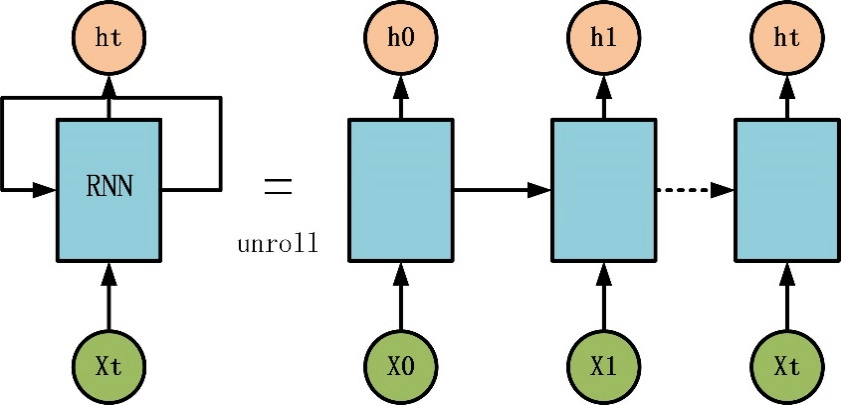
\includegraphics[scale=0.3]{figuras/intro-arq-rnn.png}
    % \caption[Así aparece el rótulo en el índice]{Así aparece el rótulo en el texto.}
    \caption[Arquitectura de red neuronal recurrente (RNN)]{\textbf{Arquitectura típica de una red neuronal recurrente, donde podemos observar la secuencia y la relación de cada celda con los estados anteriores. Fuente: \citep{articleFang2020LSTM}}}
    \label{fig-intro-arq-rnn}
\end{figure}

Precisamente esta ``memoria interna'' es lo que hace a este tipo de redes muy adecuadas para problemas de aprendizaje automático que involucran datos secuenciales. Gracias a su ``memoria interna'', las \acrshort{acr_rnn}s pueden recordar información relevante sobre la entrada que recibieron, lo que les permite ser más precisas en la predicción de lo que vendrá después, manteniendo información de contexto a diferencia de los otros tipos de redes que no pueden recordar acerca de lo que ha sucedido en el pasado, excepto lo reflejado en su entrenamiento a través de sus pesos.

Dos conceptos importantes que afectan a las \acrshort{acr_rnn} son los gradientes explosivos (\textit{exploding gradient}, en inglés) y el desvanecimiento del gradiente (\textit{vanishing gradients}, en inglés), aunque ambos efectos son propios en general de cualquier tipo de red muy grande en números de parámetros, sea o no sea recurrente. 

Estos conceptos son bien descritos por \cite{torres2019deep}, recordando que el gradiente indica el cambio a realizar en todos los pesos con respecto al cambio en el error, en tal sentido, hablamos de ``gradientes explosivos'' cuando el algoritmo asigna una importancia exageradamente alta a los pesos, sin mucha razón y esto genera un problema en el entrenamiento y hablamos de ``gradientes desaparecidos'' cuando los valores de un gradiente son demasiado pequeños y el modelo deja de aprender o requiere demasiado tiempo debido a ello. 

\subsection{Redes Long Short-Term Memory (LSTM)}
\label{section-lstm}
Como se describe en la sección anterior, las redes neuronales recurrentes convencionales presentan problemas en su entrenamiento debido a que los gradientes retropropagados tienden a crecer enormemente o a desvanecerse con el tiempo debido a que el gradiente depende no solo del error presente sino también los errores pasados. La acumulación de errores provoca dificultades para memorizar dependencias a largo plazo.

Las \acrlong{acr_lstm} (\acrshort{acr_lstm}, por sus siglas en inglés), son una extensión de las redes neuronales recurrentes, que como indica \cite{thomas2020natural}, fue propuesta por Sepp Hochreiter y Jürgen Schmidhuber en 1997 para abordar el problema de los gradientes explosivos y desaparecidos. Este tipo de redes básicamente amplían su memoria para aprender de experiencias importantes que han sido analizadas hace mucho tiempo en la secuencia. Las \acrshort{acr_lstm} permiten a las \acrshort{acr_rnn}s recordar sus entradas durante un largo período de tiempo. Esto se debe a que \acrshort{acr_lstm} contiene su información en la memoria, que puede considerarse similar a la memoria de un ordenador, en el sentido que una neurona de una \acrshort{acr_lstm} puede leer, escribir y borrar información de su memoria.

En una neurona \acrshort{acr_lstm} hay tres puertas que controlan el modo en que la información fluye dentro o fuera de la unidad: puerta de entrada (\textit{input gate}), puerta de olvidar (\textit{forget gate}) y puerta de salida (\textit{output gate}), como muestra la figura ~\ref{fig-intro-arq-lstm}. Estas puertas determinan si se permite o no una nueva entrada, se elimina la información porque no es importante o se deja que afecte a la salida en el paso de tiempo actual.

\begin{figure}[ht!]
    \centering
    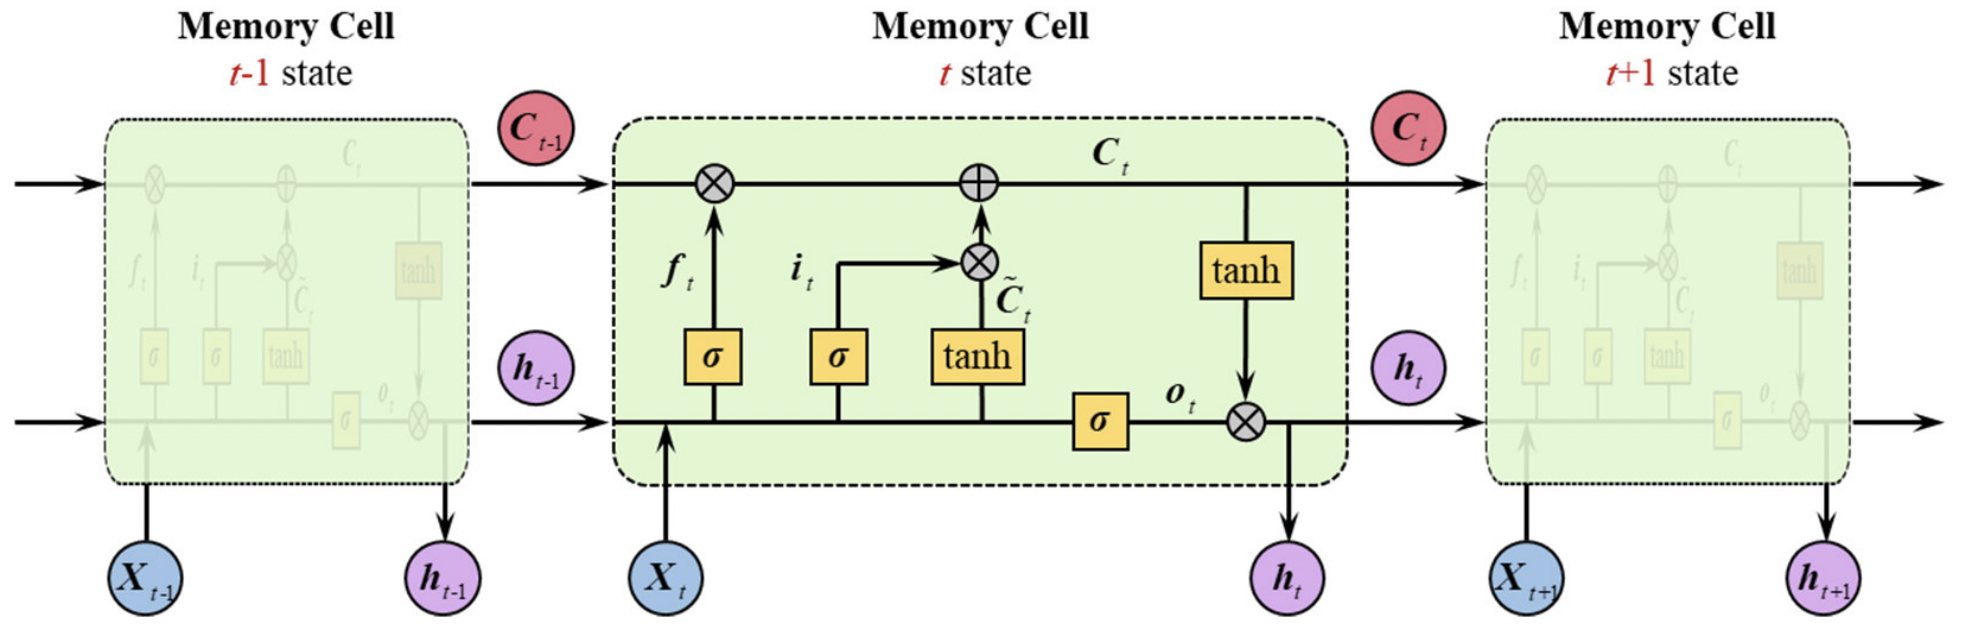
\includegraphics[scale=0.4]{figuras/intro-arq-lstm.png}
    % \caption[Así aparece el rótulo en el índice]{Así aparece el rótulo en el texto.}
    \caption[Arquitectura de red Long Short-Term Memory (LSTM)]{\textbf{Mirada interna a una celda de memoria en una red de tipo Long Short-Term Memory (LSTM). En la imagen se pueden observar los tres tipos de puertas presentes en la neurona. Fuente: \citep{LSTM_Olah_2015}}}
    \label{fig-intro-arq-lstm}
\end{figure}

\section{Bidirectional Encoder Representations from Transformer}
\label{section-bert}

\textbf{BERT} siglas para \textit{\textbf{B}idirectional \textbf{E}ncoder \textbf{R}epresentations from \textbf{T}ransformers} es un poderoso modelo de lenguaje publicado por investigadores de Google en octubre de 2018 que usa dos etapas, el preentrenamiento y el ajuste fino (\textit{fine-tunning}, en inglés), para crear modelos muy eficientes capaces de resolver  una amplia gama de tareas relacionadas al procesamiento de lenguaje natural \citep{https://doi.org/10.48550/arxiv.1810.04805}.

Desde su aparición BERT ha causado revuelo en la comunidad del \textit{machine learning} producto de su característica arquitectura que permite que el mismo modelo preentrenado se pueda ajustar para resolver una variedad de tareas finales que pueden no ser similares a las tareas para las que en un principio se entrenó y obtener resultados similares a los que definen el estado del arte para estas tareas en el campo del \acrshort{acr_nlp} (ver figura \ref{fig-intro-bert-transfer}), lo que define el objetivo principal de este trabajo (ver sección \ref{section-objetivo-general}). Los modelos como BERT y sus similares han superado varios puntos de referencia importantes en tareas de procesamiento de lenguaje natural. 

\begin{figure}[ht!]
    \centering
    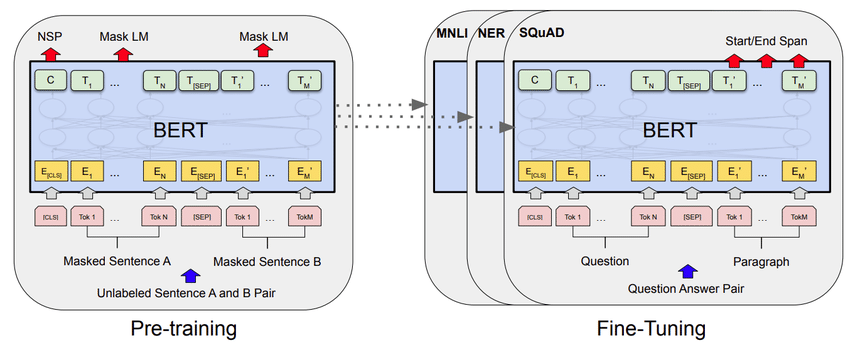
\includegraphics[scale=0.5]{figuras/intro-bert-transfer.png}
    % \caption[Así aparece el rótulo en el índice]{Así aparece el rótulo en el texto.}
    \caption[BERT - Transfer Learning]{\textbf{Procedimientos generales de preentrenamiento y fine-tunning en BERT. BERT utiliza la misma arquitecturas tanto en el preentrenamiento como en el fine-tuning. Los parámetros del modelo preentrenado se utilizan para inicializar modelos para resolver otras tareas. Fuente: \citep{https://doi.org/10.48550/arxiv.1810.04805}}}
    \label{fig-intro-bert-transfer}
\end{figure}

\subsection{Mecanismos de Atención y Transformer}
\label{subsection-atencion-transformer}

La base de BERT es el modelo \Gls{gls_transformer}, un tipo de red neuronal propuesta recientemente, basada en mecanismos de atención, que acepta como entrada datos secuenciales (por ejemplo, una secuencia de palabras) y produce algún resultado (por ejemplo, la predicción de sentimientos). A diferencia de las redes recurrentes tradicionales, como las LSTM, que procesan cada elemento de secuencia uno a la vez, con \Gls{gls_transformer} se procesan todos los elementos simultáneamente (autoatención) formando conexiones directas entre todos los elementos. Esto no solo permite una mayor paralelización, sino que también da como resultado una mayor precisión en una variedad de tareas, lo que le ha permitido impulsar importantes avances en el procesamiento del lenguaje natural.

\begin{figure}[ht!]
    \centering
    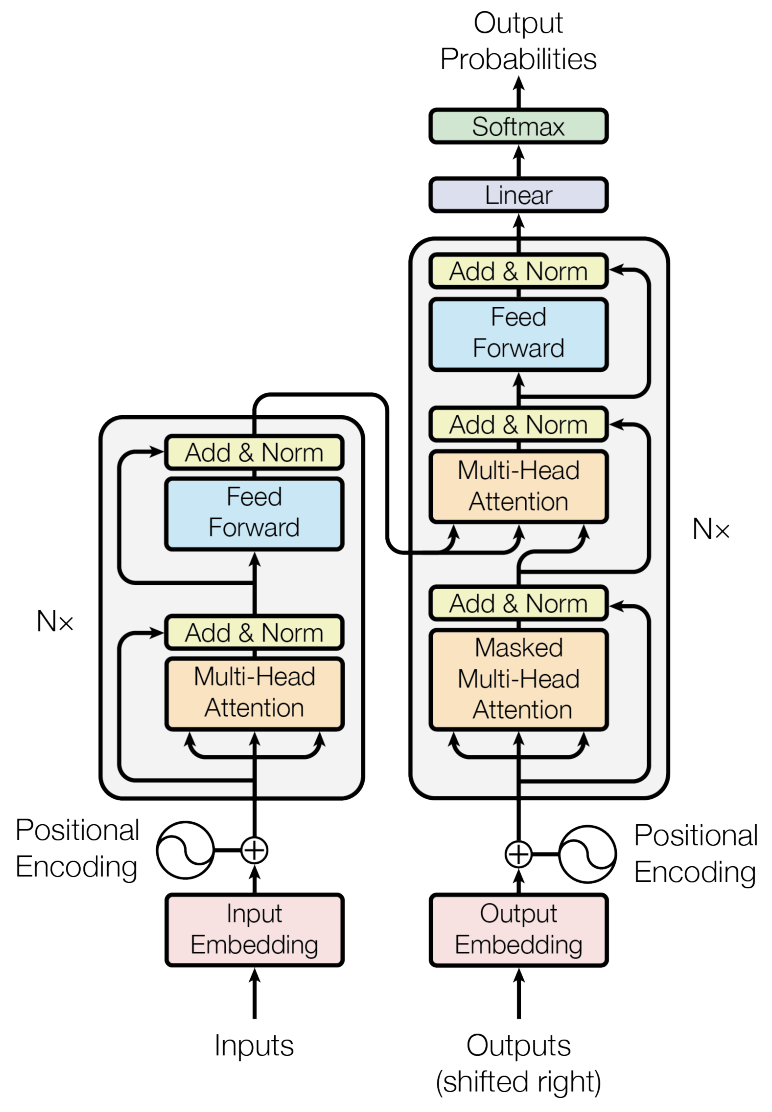
\includegraphics[scale=0.8]{figuras/intro-bert-transformers.png}
    % \caption[Así aparece el rótulo en el índice]{Así aparece el rótulo en el texto.}
    \caption[BERT - Arquitectura de Transformer]{\textbf{Arquitectura del modelo Transformer propuesto en el \textit{paper} ``Attention is all you need!''. Fuente: \citep{https://doi.org/10.48550/arxiv.1706.03762}}}
    \label{fig-intro-bert-transformers}
\end{figure}

La publicación del \textit{paper} \textit{``Attention is all you need''} \citep{https://doi.org/10.48550/arxiv.1706.03762} representó una completa revolución en el campo del procesamiento del lenguaje natural. En este \textit{paper} se propone por primera vez la arquitectura \Gls{gls_transformer} (figura \ref{fig-intro-bert-transformers}). La clave de esta novedosa arquitectura es el mecanismo de autoatención y el uso de autoencoders para lograr un entrenamiento más ágil y producir resultados eficientes. En la actualidad, años después de la publicación del \textit{paper}, esta arquitectura sigue siendo estado del arte en el mundo del NLP y la base de implementaciones como BERT o GPT.

Aunque las \acrshort{acr_rnn}s permiten observar palabras anteriores de la secuencia, sufren de memoria cortoplacista. Esto provoca que cuando trabajamos con una secuencia larga las \acrshort{acr_rnn}s no pueden observar palabras muy antiguas. Las \acrshort{acr_lstm}s tienen una ventana de memoria más grande que las \acrshort{acr_rnn}s, pero siguen teniendo una capacidad limitada. Esta secuencialidad es un obstáculo para la paralelización del proceso. Además, cuando estas secuencias son demasiado largas, el modelo tiende a olvidar el contenido de las posiciones distantes en la secuencia o a mezclarlo con el contenido de las posiciones siguientes. El mecanismo de autoatención resuelve esto ya que, permiten modelar dependencias sin considerar su distancia en las secuencias de entrada o salida. En la mayoría de los casos los mecanismos de atención se utilizan en conjunto con una red recurrente.

El Transformer utiliza dos tipos diferentes de funciones de atención (figura \ref{fig-intro-bert-attention}):
\begin{itemize}
    \item \textbf{Atención de producto punto escalado} o \textit{scaled dot-product attention}, que calcula la función de atención en un conjunto de consultas simultáneamente, empaquetadas en una matriz. 
    \item \textbf{Atención Multi-Cabeza} o \textit{Multi-Head Attention}, que permite que el modelo atienda de manera conjunta la información de diferentes subespacios de representación en diferentes posiciones.
\end{itemize}

\begin{figure}[ht!]
    \centering
    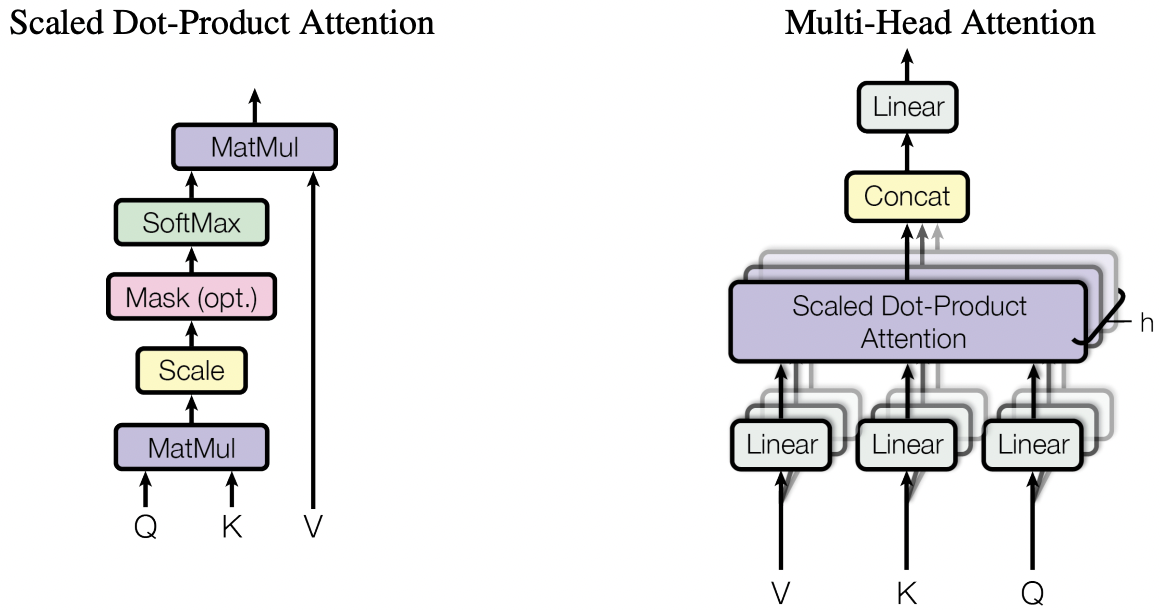
\includegraphics[scale=0.7]{figuras/intro-bert-attention.png}
    % \caption[Así aparece el rótulo en el índice]{Así aparece el rótulo en el texto.}
    \caption[BERT - Mecanismos de Atención]{\textbf{A la izquierda podemos observar el mecanismo de atención basado en el producto punto escalado y a la derecha el mecanismo de atención multi-head, el cual consiste en varias capaz de atención corriendo en paralelo. Fuente: \citep{https://doi.org/10.48550/arxiv.1706.03762}}}
    \label{fig-intro-bert-attention}
\end{figure}

En cuanto a las entradas, el \textit{paper} de \cite{https://doi.org/10.48550/arxiv.1706.03762} menciona que las secuencias de entrada se representan utilizando alguna forma de \gls{gls_wordembeddings}, es decir, una representación vectorial de cada palabra que guarda información semántica. Esto se hace tanto para el \textit{encoder} como para el \textit{decoder}. Los \gls{gls_wordembeddings} por sí solos carecen de cualquier información posicional que se logra en las \acrshort{acr_rnn}s en virtud de su naturaleza secuencial. Mientras tanto, en la autoatención se pierde cualquier información posicional debido a la aplicación de la función \gls{gls_softmax}. Para preservar la información posicional, el \Gls{gls_transformer} inyecta un vector a los embeddings de entrada individuales. Este vector inyectado se denomina ``codificación posicional'' y se agrega a los \textit{embeddings} de entrada en la parte inferior de las pilas del \textit{encoder} y \textit{decoder}.

Los autores compararon los resultados de la arquitectura con otras soluciones consideradas estado del arte en 2017. La arquitectura \Gls{gls_transformer} obtuvo un desempeño mejor que el de otros modelos. (figura \ref{fig-intro-bert-transresults}) 

\begin{figure}[ht!]
    \centering
    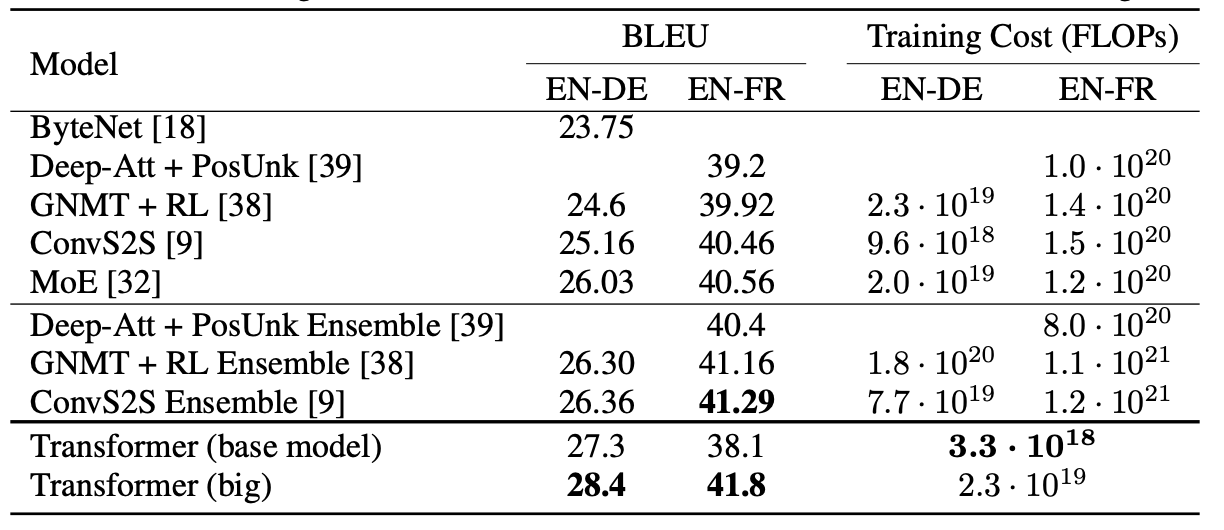
\includegraphics[scale=0.6]{figuras/intro-bert-transresults.png}
    % \caption[Así aparece el rótulo en el índice]{Así aparece el rótulo en el texto.}
    \caption[BERT - Transformer Resultados]{\textbf{La imagen compara el resultado de la implementación de la arquitectura \Gls{gls_transformer} en un problema de traducción superando el desempeño de otros modelos considerados el estado del arte antes de la publicación del \textit{paper} ``All you Need is Attention''. En la comparación se observa además de un mejor desempeño, un costo de procesamiento menor al del resto de modelos. Fuente: \cite{https://doi.org/10.48550/arxiv.1706.03762}}}
    \label{fig-intro-bert-transresults}
\end{figure}

\subsection{Arquitectura de BERT}
\label{subsection-arquitectura-bert}

La arquitectura de BERT es básicamente una pila de \textit{encoders} de la arquitectura \Gls{gls_transformer}. 

En el \textit{paper} original de BERT \cite{https://doi.org/10.48550/arxiv.1810.04805} hablan de dos modelos o versiones de BERT que se pueden elegir en términos de implementación:

\begin{itemize}
    \item \textbf{BERT$_{BASE}$:} L=12, H=768, A=12, 110 millones de parámetros.
    \item \textbf{BERT$_{LARGE}$:} L=24, H=1024, A=16, 340 millones de parámetros.
\end{itemize}

donde:\\
L: número de capas de encoders\\
H: tamaño de la capa oculta (dimensión del embedding)\\
A: número de encabezados de auto atención\\

La innovación técnica clave de BERT es aplicar el entrenamiento bidireccional de \Gls{gls_transformer} al modelamiento del lenguaje. Esto es diferente a los enfoques de modelos anteriores que analizaban las secuencias de texto en una sola dirección. Los resultados obtenidos por \cite{https://doi.org/10.48550/arxiv.1810.04805} en su \textit{paper}, muestran que un modelo de lenguaje entrenado bidireccionalmente tiene un sentido más profundo del contexto y flujo del lenguaje que los modelos de lenguaje de una sola dirección. 

El preentrenamiento de BERT está basado en dos tareas no supervisadas:

\begin{enumerate}
    \item \textbf{Modelo de Lenguaje Enmascarado} o \textit{Masked Language Model} (MLM): esta tarea es la que habilita el aprendizaje bidereccional profundo en el modelo. En esta tarea se enmascara un porcentaje de los tokens de entrada (reemplazando los tokens por el token especial [MASK]) al azar y el modelo intenta predecir los tokens que han sido enmascarados. Esos tokens predichos del modelo luego son introducidos a una función softmax de salida sobre el vocabulario para obtener las palabras de salida finales.
    \item  \textbf{Predicción de la Siguiente Oración} o \textit{Next Sentence Prediction} (NSP): esta tarea es la utilizada para que el modelo sea capaz de resolver tareas donde es importante la relación entre dos oraciones. En este caso, el modelo es entrenado recibiendo pares de frases como entrada y aprendiendo a predecir si la segunda frase del par es la subsiguiente dentro del documento original de entrada.
\end{enumerate}

El modelo esta entrenado en ambas tareas mencionadas anteriormente de forma simultánea. Esto es posible debido a la forma en la que el modelo procesa las entradas y las salidas, las cuales son compatibles para ambos problemas. 

En cuanto a la entrada (ver figura \ref{fig-intro-bert-transresults}), BERT necesita recibir información tanto para una sola oración como para dos oraciones agrupadas sin ambigüedades en una secuencia de token. Los autores del \textit{paper} oficial señalan que una secuencia de entrada puede ser un tramo arbitrario de texto contiguo, en lugar de una oración lingüística real. El token [SEP] se usa para separar dos oraciones.

A diferencia de las \acrshort{acr_rnn}s en las que las entradas se alimentan secuencialmente, el modelo BERT no puede conservar el orden de los tokens de entrada. El orden de las palabras en cada idioma es significativo, tanto semántica como sintácticamente. Para realizar correctamente la tarea de predicción de la siguiente oración, el modelo debe ser capaz de distinguir entre las dos oraciones. Ambos problemas se resuelven agregando \textit{embeddings} que contienen la información requerida a los tokens correspondientes a la entrada original y usando el resultado como entrada a nuestro modelo BERT. 

\begin{figure}[ht!]
    \centering
    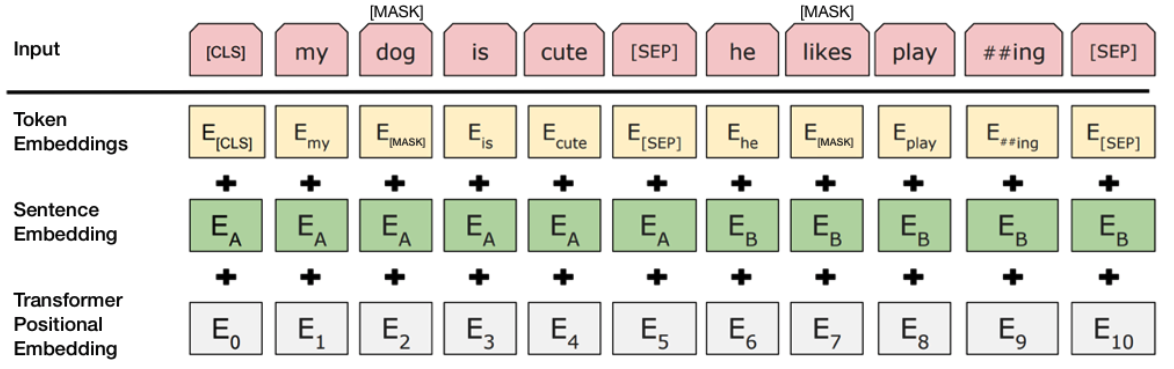
\includegraphics[scale=0.3]{figuras/intro-bert-tokens.png}
    % \caption[Así aparece el rótulo en el índice]{Así aparece el rótulo en el texto.}
    \caption[BERT - Token Embeddings]{\textbf{Representación de la entrada del modelo de BERT. El input del modelo es la suma de los token embeddings, el embedding de segmentación y el embedding posicional. Fuente: \cite{https://doi.org/10.48550/arxiv.1706.03762}}}
    \label{fig-intro-bert-tokens}
\end{figure}

Los siguientes \textit{embeddings} se agregan a los \textit{embeddings} de tokens:

\begin{itemize}
    \item \textbf{Embedding de segmentos} o \textit{Segment Embedding}: Proporciona información sobre la oración de la que forma parte un token en particular.
    \item  \textbf{Embedding posicional} o \textit{Position Embedding}: Proporciona información sobre el orden de las palabras de entrada.
\end{itemize}

En cuanto a la salida, también está diseñada para predecir el resultado de dos tareas diferentes de forma simultánea. Esto lo hace mediante el uso de diferentes capas \acrshort{acr_ffnn} y \gls{gls_softmax} construidas sobre las salidas del último \textit{encoder}. El primer token de entrada es siempre un token de clasificación especial [CLS]. El estado final correspondiente a este token se usa como la representación de secuencia agregada para las tareas de clasificación y se usa para la predicción de la siguiente oración. Los estados finales correspondientes a los tokens [MASK] se introducen en la \acrshort{acr_ffnn} y \gls{gls_softmax} para predecir la siguiente palabra del vocabulario.

\subsection{BERT y Fine Tunning}
\label{subsection-bert-finetunning}

La idea de la transferencia de aprendizaje o \textit{transfer learning} (en inglés), es entrenar un modelo en una tarea y luego aprovechar el conocimiento adquirido para mejorar el rendimiento del modelo en una tarea relacionada. El \textit{fine-tunning} es un enfoque para transferir el aprendizaje en el que se agrega una capa a la salida del modelo para que se ajuste a una nueva tarea y se entrena el modelo resultante.

Una consecuencia positiva de agregar capas (entrada/salida) y no cambiar el modelo BERT es que solo se necesita aprender una cantidad mínima de parámetros desde cero, lo que hace que el procedimiento sea rápido, rentable y eficiente en recursos.

En la clasificación de pares de oraciones y la clasificación de oraciones únicas, el estado final correspondiente al token [CLS] se usa como entrada para las capas adicionales que hacen la predicción. (ver figura \ref{fig-intro-bert-finetunning})

\begin{figure}[ht!]
    \centering
    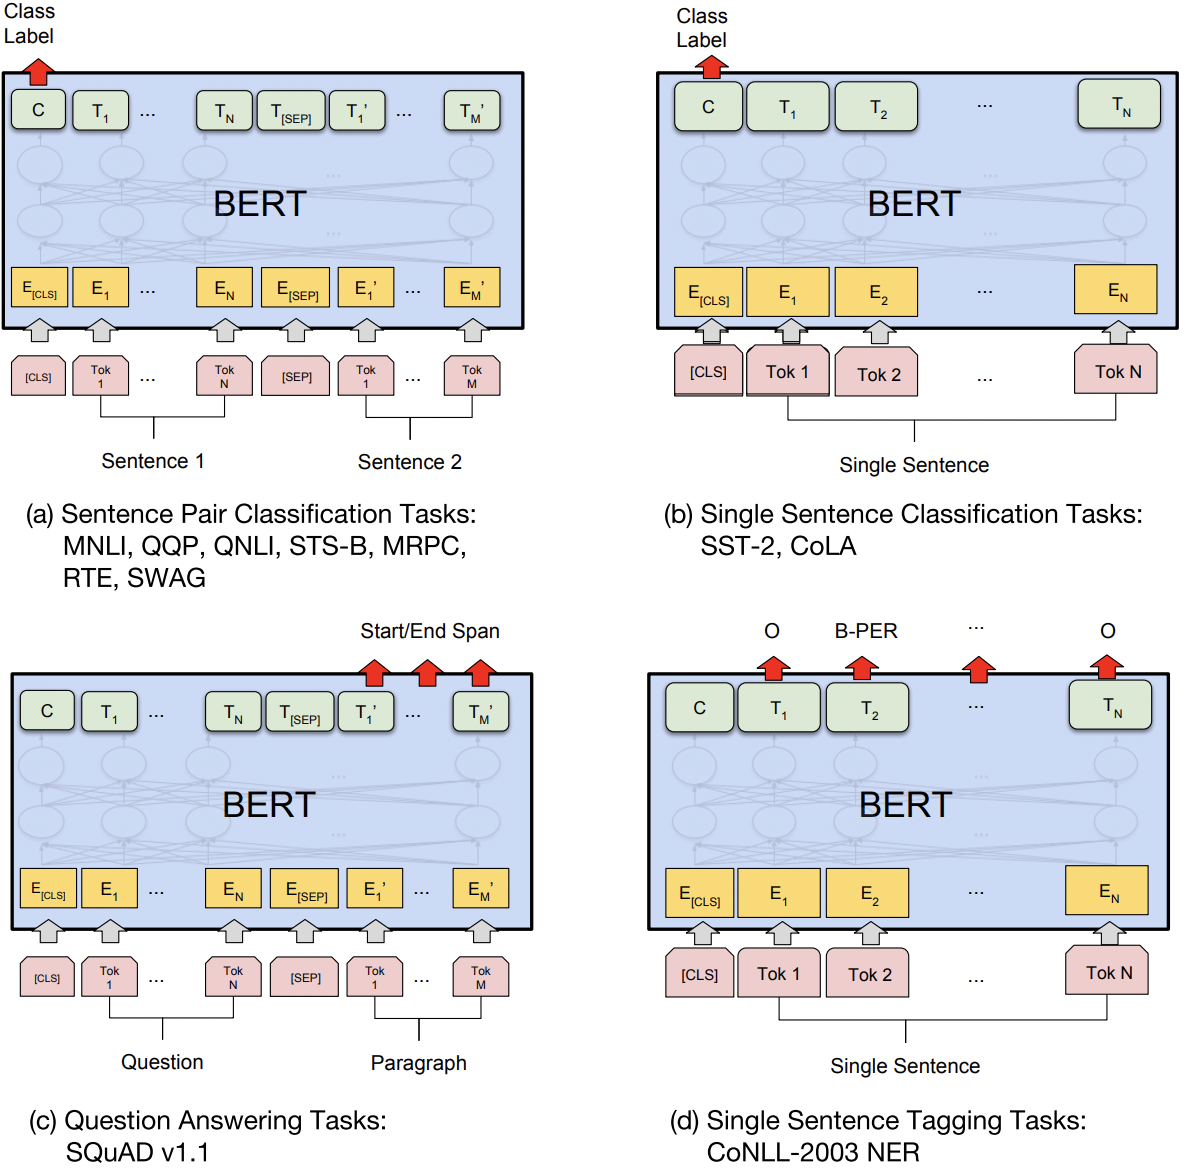
\includegraphics[scale=0.6]{figuras/intro-bert-finetunning.png}
    % \caption[Así aparece el rótulo en el índice]{Así aparece el rótulo en el texto.}
    \caption[BERT - Fine-tunning]{\textbf{Esta imagen ilustra el proceso de fine-tunning para BERT en diferentes tareas y como se amolda la arquitectura unificada para distintas tareas. Fuente: \cite{https://doi.org/10.48550/arxiv.1706.03762}}}
    \label{fig-intro-bert-finetunning}
\end{figure}

En las tareas de preguntas y respuestas, se introducen un vector de inicio (S) y uno final (E) durante el \textit{fine-tunning}. La pregunta se introduce al modelo como oración A y la respuesta como oración B. La probabilidad de que la palabra i sea el comienzo del intervalo de respuesta se calcula como un producto escalar entre Ti (estado final correspondiente al i-ésimo token de entrada) y S (vector de inicio) seguido por un \textit{softmax} sobre todas las palabras del párrafo. Se utiliza un método similar para el tramo final. (ver figura \ref{fig-intro-bert-finetunning})

Entre las ventajas del proceso de \textit{fine-tunning} podemos mencionar:

\begin{itemize}
    \item \textbf{Desarrollo más rápido}
En primer lugar, los pesos del modelo BERT preentrenados ya codifican mucha información sobre el lenguaje. Como resultado, lleva mucho menos tiempo entrenar el modelo ajustado, es como si ya se hubiera entrenado las capas inferiores de nuestra red de forma exhaustiva y solo se necesita ajustar levemente mientras se usa su salida como características para la tarea de clasificación. De hecho, los autores recomiendan solo de 2 a 4 épocas de entrenamiento para ajustar BERT en una tarea específica de NLP, en comparación con los cientos de horas de \acrlong{acr_gpu} (\acrshort{acr_gpu}, por sus siglas en inglés) necesarias para entrenar el modelo BERT original o una LSTM desde cero.
\item \textbf{Menos datos}
Además, y quizás igual de importante, debido a los pesos previamente entrenados, este método permite ajustar una tarea en un conjunto de datos mucho más pequeño que el que se requeriría en un modelo construido desde cero. Un inconveniente importante de los modelos NLP creados \textit{from scratch} es que a menudo se requiere de un conjunto de datos prohibitivamente grande para entrenar nuestra red con una precisión razonable, lo que significa que se tiene que dedicar mucho tiempo y energía a la creación del conjunto de datos. Al ajustar BERT, ahora se puede entrenar un modelo para que tenga un buen rendimiento con una cantidad mucho menor de datos de entrenamiento.
\item \textbf{Mejores resultados}
Finalmente, se demostró que este sencillo procedimiento de ajuste fino (por lo general, agregar una capa completamente conectada encima de BERT y entrenar durante algunas épocas) logra resultados de vanguardia con ajustes mínimos específicos de tareas para una amplia variedad de tareas: clasificación, inferencia de lenguaje, similitud semántica, respuesta a preguntas, etc. En lugar de implementar arquitecturas personalizadas, se ha demostrado que funciona bien en una tarea específica, simplemente ajustar BERT. Esta opción se muestra como una alternativa mejor (o al menos igual).
\end{itemize}

\subsection{BERT, variantes y otros modelos}
\label{subsection-bert-otros}

BERT no es el único modelo que está produciendo estos resultados innovadores. Existe otro modelo desarrollado por OpenAI llamado GPT-3 \citep{articleBrownGPT3} que está causando bastante revuelo en el mundo del NLP.  

GPT ha causado bastante revuelo en Internet últimamente. Este modelo tiene algo en común con BERT, y es que ambos modelos reutilizan un componente de \Gls{gls_transformer}. Como se indicó anteriormente, BERT apila la parte del encoder del \Gls{gls_transformer} como su bloque de construcción. Mientras tanto, GPT usa la parte del decoder del \Gls{gls_transformer} como su bloque de construcción.

Las conexiones bidireccionales en BERT se deben a la autoatención bidireccional del \textit{encoder}. Mientras tanto, las conexiones en GPT solo están en una sola dirección, de izquierda a derecha, debido al diseño del \textit{decoder} para evitar mirar predicciones futuras.

Adicionalmente, hay algunas variantes de BERT donde la arquitectura no es diferente, pero presentan ciertas adecuaciones. (ver tabla \ref{tbl-bert-variants}) 

Paste Latex Here\begin{table}[ht!]
\resizebox{\textwidth}{!}{
	\begin{tabular}{l|c|p{9cm}}
		\toprule
		\textbf{Modelo}                                                         & \textbf{Creador} & \textbf{Descripción}                                                                                                                                                                                                                                                                                                                          \\ \midrule
		Albert \cite{ALBERT_https://doi.org/10.48550/arxiv.1909.11942}          & Google           & Este paper describe técnicas de reducción de parámetros para disminuir la reducción de memoria y aumentar la velocidad de entrenamiento de los modelos BERT.                                                                                                                                                                               \\ \midrule
		RoBERTa \cite{ROBERTA_https://doi.org/10.48550/arxiv.1907.11692}        & Facebook         & Este paper cree que los modelos BERT originales estaban poco entrenados y muestra que con más entrenamiento/ajuste puede superar los resultados iniciales.                                                                                                                                                                                    \\ \midrule
		ERNIE \cite{ERNIE_https://doi.org/10.48550/arxiv.1904.09223}            & -                & Representación mejorada a través de la integración del conocimiento de Baidu: se inspira en la estrategia de enmascaramiento de BERT y aprende la representación del lenguaje mejorada mediante estrategias de enmascaramiento del conocimiento, que incluyen el enmascaramiento a nivel de entidad y el enmascaramiento a nivel de frase. \\ \midrule
		DistilBERT  \cite{DISTILBERT_https://doi.org/10.48550/arxiv.1910.01108} & -                & BERT más pequeño. Reduce el número de capas a 6 y elimina el embedding de segmentación                                                                                                                                                                                                                                                     \\ \bottomrule
	\end{tabular}
}
% \caption[Así aparece el rótulo en el índice]{Así aparece el rótulo en el texto.}
\caption[BERT - Otros modelos de lenguaje basados en BERT]{\textbf{Lista de modelos basados en BERT. Fuente: \cite{articleBrownGPT3}}}
\label{tbl-bert-variants}
\end{table}
% OBJETIVOS

\cleardoublepage

\chapter{Objetivos}
\label{chapter-objetivos}

La publicación de BERT por parte de Google marcó el inicio de una nueva era en el machine learning obteniendo con este modelo excelentes resultados que definieron un nuevo estado del arte en muchas tareas y benchmarks en el campo del procesamiento de lenguaje natural.

El hecho de ser un modelo accesible, con una arquitectura unificada que permite un ajuste rápido y fácil, lo convierte en un modelo de referencia.

\section{Objetivo General}
\label{section-objetivo-general}

Basado en los fundamentos antes expuestos, el objetivo principal de este trabajo es: \textbf{Evaluar el uso y desempeño de BERT (Biderectional Encoder Representations for Transformers) como modelo en la resolución de tareas relacionadas al procesamiento del lenguaje natural, distintas a las que para en un principio fue preentrenado.} Específicamente, se trabajará en dos tareas, el análisis de sentimiento y el problema de respuesta a preguntas.
\medskip

\section{Objetivo Específicos}
\label{section-objetivos-especificos}

Para evaluar el uso y desempeño de este modelo en la resolución de problemas asociados al procesamiento de lenguaje natural, trabajaremos en los objetivos específicos citados a continuación:
\medskip

\begin{enumerate}[label=\destacado{\arabic*.}]
  \setlength\itemsep{1em}
  \item Identificar problemas típicos del procesamiento del lenguaje natural donde, el uso de modelos basados en \textit{transformers} hayan tenido un aporte considerable en su solución.

  \item Identificar y seleccionar un conjunto de datos para cada tarea que permita construir una solución a través del ajuste del modelo. Estudiar, limpiar y dividir los datos en los subconjuntos de entrenamiento, prueba y validación.

  \item Evaluar el estado del arte para cada uno de estos problemas, entendiendo el desempeño de distintos algoritmos empleados en su solución.
  
  \item Desarrollar soluciones basadas en el ajuste de BERT, adecuándose para resolver los problemas seleccionados.
  
  \item Comparar el desempeño de las soluciones desarrolladas con el estado del arte haciendo uso de las métricas apropiadas en cada benchmark.
\end{enumerate}
% METODOLOGÍA

\cleardoublepage

\chapter{Metodología y Desarrollo}
\label{chapter-metodologia-desarrollo}

La idea general del \textit{transfer learning} es preentrenar un modelo usando una red neuronal de gran tamaño sobre un dataset de gran volumen para después ajustar la red (\textit{fine-tunning}) usando un dataset mucho más reducido y ajustado a la tarea especifica que se intenta resolver. El aprendizaje por transferencia marca una gran diferencia y nos permite resolver nuevos problemas mucho más fácilmente, ya que normalmente podemos cargar pesos previamente entrenados de un modelo sin requerir de un gran conjunto de datos para resolver una tarea específica.

BERT es un modelo de lenguaje preentrenado que ha demostrado que el concepto de la transferencia del aprendizaje ha resultado ser una herramienta poderosa no solo en los problemas de visión por computacdora (\gls{gls_computer_vision}, en inglés), sino también en el procesamiento natural del lenguaje y que podría ser suficiente con un ligero ajuste (\textit{fine-tunning}) implementar un nuevo modelo que resuelva de forma satisfactoria  una nueva tarea.

El \textit{transfer learning} se convirtió en la estrategia predeterminada en la visión por computadora alrededor del año 2014. A menudo usaban modelos que estaban entrenados previamente para la clasificación de imágenes en Imagenet \cite{Olga2015Imagenet}, lo que significaba que usaban aprendizaje supervisado y un gran conjunto de datos con etiquetas para entrenar previamente el modelo. Durante varios años se estuvo investigando sin éxito formas de usar el aprendizaje por transferencia en el procesamiento del lenguaje natural y se estuvo tratando de encontrar tareas y conjuntos de datos con las mismas propiedades atractivas que tenía Imagenet para la visión por computadora. Finalmente, en 2018 al menos tres artículos diferentes (BERT \cite{https://doi.org/10.48550/arxiv.1810.04805}, ELMo \cite{Peters2018Elmo}, GPT \cite{radford2018improving}) demostraron que se puede usar el \textit{transfer learning} también en el procesamiento natural del lenguaje. 

Entre estos modelos, se puede decir que BERT fue el más limpio, ya que requirió la menor cantidad de \textit{fine-tunning}, un conjunto de datos más pequeño y, en general, también dio los mejores resultados.

Basados en estos conceptos de \textit{transfer learning} y \textit{fine-tunning} procederemos a evaluar el uso y el desempeño de BERT en la resolución de problemas de procesamiento natural del lenguaje siguiendo los siguientes pasos:

\begin{enumerate}
  \item \textbf{Selección de problemas} \\
  En esta primera etapa elegimos un par de problemas típicos del procesamiento natural del lenguaje pero que a su vez sean distintos a los problemas para los que BERT fue entrenado inicialmente. La idea es poder demostrar la adaptabilidad del modelo para resolver cualquier clase de problemas basado en la arquitectura propia de BERT. Los problemas con los que trabajaremos son el Análisis de Sentimiento (clasificación) y la tarea de Respuesta a Preguntas.
  \item \textbf{Selección de los conjuntos de datos (\textit{datasets})} \\
  En cuanto a la selección de los \textit{datasets} se decidió trabajar con conjuntos de datos asociados a cada uno de los problemas antes descritos, procurando que los \textit{datasets} elegidos permitan establecer indicadores de comparación y que existan estudios de comparación del desempeño con otros modelos y soluciones. Para el caso de análisis de sentimiento se trabajará con un \textit{dataset} de reseñas de películas de IMDB creado por investigadores de la Universidad de Stanford, para el problema de preguntas y respuestas se trabajó con el conocido \textit{dataset} SQuAD en su versión 1.0.
  \item \textbf{Fine Tuning de BERT} \\
  Para cada uno de los problemas elegidos se hizo un ajuste del modelo inicial de BERT usando para el entrenamiento un \textit{dataset} etiquetado. La intención es hacer las adecuaciones necesarias al modelo para intentar encontrar una solución simple a cada uno de los problemas elegidos.
  \item \textbf{Evaluación de los resultados} \\
  Se compararon los resultados obtenidos en cada problema con otros modelos implementados para resolver el problema. La idea es validar que simplemente haciendo un pequeño \textit{fine-tunning} del modelo original podemos obtener resultados similares o cercanos a los del estado del arte en cada problema.
\end{enumerate}

\clearpage 
%%%%%%%%%%%%%%%%%%%%%%%%%%%%%%%%%%%%%
% SECTION - ANÁLISIS DE SENTIMIENTO 
%%%%%%%%%%%%%%%%%%%%%%%%%%%%%%%%%%%%%

\section{Problema de Análisis de Sentimiento (Clasificación)}
\label{section-analisis-de-sentimiento}

%%%%%%%%%%%%%%%%%%%%%%%%%%%%%%%%%%%%%%%%%%%%%%%%%%%%%%%%%%%%%%%%%%%%%%%%%%%%%%%%%%%%%%%%%%%%%%%%%%%%%%%%%%%%%%%

\subsection{Descripción del problema}
\label{subsection-as-descripcion-problema}

El análisis de sentimiento es un subcampo del procesamiento de lenguaje natural que ha tenido un gran desarrollo en los últimos años. Este interés ha sido alimentado en gran parte por el auge de las redes sociales que ha dado lugar a la aparición de blogs, foros y aplicaciones en línea que le permiten a los usuarios discutir sobre cualquier tema y compartir sus opiniones. Este tipo de análisis es ampliamente usado por distintas empresas para entender la opinión de sus clientes y conocer la aceptación de sus productos y servicios. 

A través del análisis de sentimiento las empresas pueden estudiar los comentarios de los clientes para prestar una mejor atención, crear mejores productos o mejorar sus estrategias de marketing para atraer nuevos clientes. En líneas generales los resultados del análisis de sentimiento ayudan a conocer mejor los intereses y opiniones de los clientes sobre las tendencias del mercado.

El objetivo principal del problema es analizar una secuencia de texto y a partir de ella identificar o extraer información subjetiva que permita inferir si el sentimiento asociado a la frase es positivo o negativo. Desde otro punto de vista, se trata de una tarea de clasificación de la polaridad asociada a los textos que pueden estar presentes en documentos, oraciones u opiniones de forma masiva y automática. 

En el estudio de \cite{Bhavitha_sa}, los autores señalan que las técnicas de análisis de sentimientos se pueden clasificar en tres enfoques distintos en cuanto a la forma de solución.
\begin{enumerate}
  \item \textbf{Enfoque de aprendizaje automático:} Cuando utilizamos modelos de \textit{machine learning} en la solución del problema y generalmente nos basamos en un modelo especifico a partir del entrenamiento sobre un gran corpus de documentos.
  \item \textbf{Enfoque basados en léxico:} Mediante este enfoque, la orientación semántica de las palabras de un texto se calcula obteniendo las polaridades de las palabras a partir de un léxico predefinido. Es decir, habrá palabras en el texto que por si sola denotan ya una polaridad. Ejemplo, palabras como \textit{magnifico, bueno, grandioso, espectacular}, tienen un sentido positivo, mientras que palabras como \textit{horrible, malo, decepción}, tienen un significado negativo.
  \item \textbf{Enfoque híbrido:} Se basa en la combinación de información lingüística y estadística, reglas semánticas junto con el uso de redes neuronales profundas.
\end{enumerate}

Más recientemente, se utilizan técnicas de aprendizaje profundo, como BERT, T5 y GPT, para entrenar clasificadores de sentimientos de alto rendimiento que se evalúan mediante métricas como F1, recuperación y precisión. 

%%%%%%%%%%%%%%%%%%%%%%%%%%%%%%%%%%%%%%%%%%%%%%%%%%%%%%%%%%%%%%%%%%%%%%%%%%%%%%%%%%%%%%%%%%%%%%%%%%%%%%%%%%%%%%%

\subsection{Selección del Dataset}
\label{subsection-as-dataset-imdb}

Para evaluar los sistemas de análisis de sentimientos, se utilizan generalmente conjuntos de datos de referencia como:

\begin{itemize}
    \item \textbf{SST (Stanford Sentiment Treebank):} es un corpus con árboles de análisis sintáctico completamente etiquetados que permite un análisis completo de los efectos compositivos del sentimiento en el lenguaje. El corpus se basa en el conjunto de datos presentado por \citep{PANG_LEE_SST_https://doi.org/10.48550/arxiv.cs/0506075} y consta de 11.855 oraciones individuales extraídas de reseñas de películas. Se analizó con el analizador de Stanford e incluye un total de 215154 frases únicas de esos árboles de análisis, cada una anotada por 3 jueces humanos.
    Cada frase está etiquetada como negativa, algo negativa, neutral, algo positiva o positiva. El corpus con las 5 etiquetas se denomina SST-5 o SST de grano fino. Los experimentos de clasificación binaria en oraciones completas (negativas o algo negativas versus algo positivas o positivas con oraciones neutras descartadas) se refieren al conjunto de datos como SST-2 o SST binario.
    
     \item \textbf{GLUE (General Language Understanding Evaluation benchmark):} es una colección de nueve tareas de comprensión del lenguaje natural, que incluyen tareas de una sola oración CoLA y SST-2, tareas de similitud y paráfrasis MRPC, STS-B y QQP, y tareas de inferencia del lenguaje natural MNLI, QNLI, RTE y WNLI.
     
     \item \textbf{Large Movie Review Dataset IMDB:} es el conjunto de datos que se seleccionó para este experimento y que se procederá a describir a continuación.
\end{itemize}

El \textit{\textbf{Large Movie Review Dataset IMDB}} es un conjunto de datos con 50.000 reseñas de películas creado para la clasificación de sentimientos binarios que contiene sustancialmente más datos que los otros conjuntos de datos de referencia.

Como describen los creadores de este \textit{dataset} en su \textit{paper} del 2019 \textit{Learning Word Vectors for Sentiment Analysis} \cite{maas-EtAl:2011:ACL-HLT2011}, este conjunto de datos fue creado a partir de reseñas de películas realizadas por la audiencia y extraídas del sitio público IMDB. Para la construcción del mismo consideraron no incluir más de 30 reseñas por película.

Este conjunto de datos se encuentra balanceado, es decir, contiene un mismo número de reseñas positivas y negativas. Los autores para construirlo consideraron solo críticas altamente polarizadas en base al sistema de rating que tiene IMDB y de esa forma consideraron una crítica negativa a aquellas reseñan que tenían una puntuación $\leq$ 4 sobre 10 y positiva si la puntuación era $\geq$ 7 sobre 10. Las reseñas neutrales no fueron incluidas

Para el propósito de este trabajo se usó una versión del \textit{dataset} original transformado y disponible en la plataforma \textit{kaggle.com} \citep{n_2019}. Esta versión ha sido transformada a un archivo de valores separados por comas, CSV (del inglés comma-separated values), en el cual se presentan dos columnas una para la reseña y otra para el sentimiento.

La razón por la que se escogió este \textit{dataset} y no otro es la amplia cantidad de soluciones desarrolladas tomando como base de entrenamiento el mismo, esto permitirá poder hacer un estudio del resultado obtenido y compararlo con otros modelos.

%%%%%%%%%%%%%%%%%%%%%%%%%%%%%%%%%%%%%%%%%%%%%%%%%%%%%%%%%%%%%%%%%%%%%%%%%%%%%%%%%%%%%%%%%%%%%%%%%%%%%%%%%%%%%%%

\subsection{Estado del arte}
\label{subsection-as-estado-del-arte}

Para evaluar el estado del arte relacionado a la solución de análisis de sentimiento sobre el \textit{dataset} de reseñas de IMDB se utilizaron diversas fuentes. 

En el trabajo de \cite{Dang_2020} los autores analizaron y realizaron una comparación entre distintos estudios que usan el aprendizaje profundo como las \acrlong{acr_dnn} (\acrshort{acr_dnn}, por sus siglas en inglés), \acrlong{acr_rnn} (\acrshort{acr_rnn}, por sus siglas en inglés) y \acrlong{acr_cnn} (\acrshort{acr_cnn}, por sus siglas en inglés), para resolver diferentes problemas asociados al análisis de sentimiento. En este estudio no se incluyeron las recién aparecidas (para ese momento) redes basadas en Transformers. Los autores usaron distintos datasets para la evaluación entre ellos el mismo utilizado en este trabajo \ref{subsection-as-dataset-imdb} y utilizaron en el preprocesamiento de los datos dos técnicas distintas de procesamiento de texto (\gls{gls_wordembeddings} y \gls{gls_tfidf}). En sus conclusiones, los autores deducen una fiabilidad ligeramente superior en la mayoría de conjunto de datos con las redes neuronales recurrentes, sin embargo, igual mencionan un tiempo de cálculo mucho más largo, como se puede evidenciar en las imágenes \ref{fig-as-eda-accuracy-comparison} y \ref{fig-as-eda-cpu-comparison} 

\begin{figure}[ht!]
    \centering
    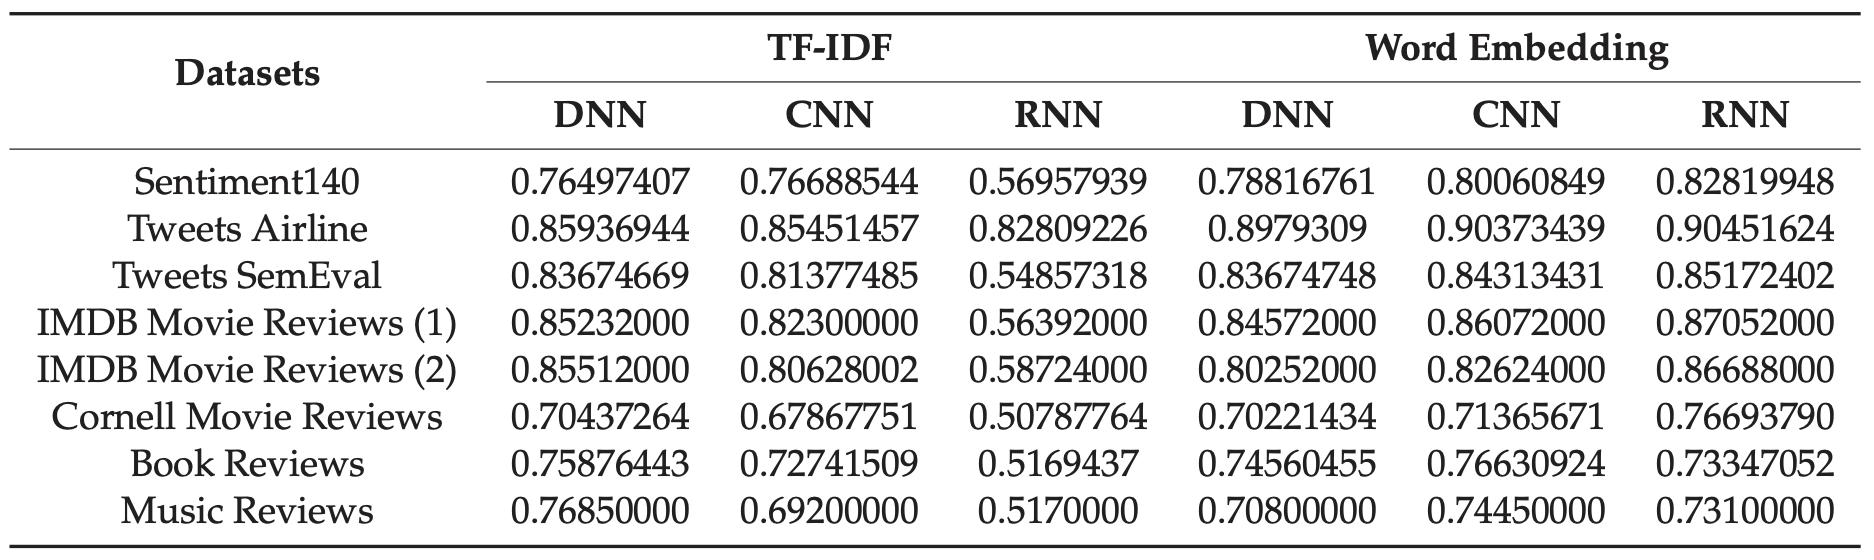
\includegraphics[scale=0.45]{figuras/as-eda-accuracy-comparison.png}
    % \caption[Así aparece el rótulo en el índice]{Así aparece el rótulo en el texto.}
    \caption[Análisis de Sentimiento - Tabla - Accuracy]{Comparación del accuracy obtenido para datasets con dos clases (positivo y negativo), en el artículo \textit{Sentiment Analysis Based on Deep Learning: A Comparative Study}. \textbf{Fuente: \cite{Dang_2020}}}
    \label{fig-as-eda-accuracy-comparison}
\end{figure}

\begin{figure}[ht!]
    \centering
    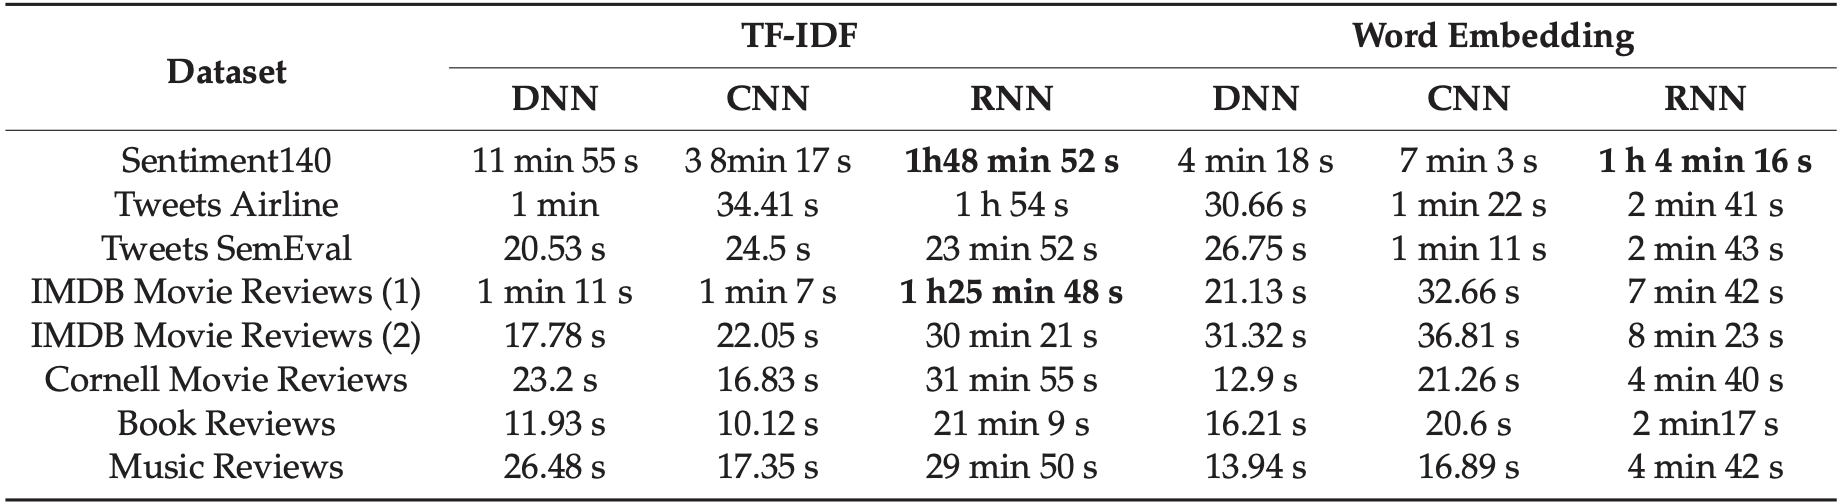
\includegraphics[scale=0.45]{figuras/as-eda-cpu-comparison.png}
    % \caption[Así aparece el rótulo en el índice]{Así aparece el rótulo en el texto.}
    \caption[Análisis de Sentimiento - Tabla - Performance]{\textbf{Comparación de los tiempos de cómputo experimentados para el entrenamiento de modelos con \acrshort{acr_gpu}, en el artículo \textit{Sentiment Analysis Based on Deep Learning: A Comparative Study}. Fuente: \cite{Dang_2020}}}
    \label{fig-as-eda-cpu-comparison}
\end{figure}

Es importante mencionar con respecto a este estudio que si bien las RNN evidenciaron tener un mejor desempeño con todos los datasets esto solo ocurrió con el uso de Word Embedding como técnica de preprocesado de los datos y no con \gls{gls_tfidf}.

Adicionalmente nos basamos en el sitio web NLP-progress (\url{https://nlpprogress.com/}) \cite{Ruder_NLP-progress_2022}, el cual es un repositorio en linea que hace un seguimiento del progreso en distintos problemas en el procesamiento del lenguaje natural NLP, incluidos los datasets y el estado del arte actual para las tareas de NLP más comunes.

Este repositorio muestra un ranking de modelos \ref{tbl-nlpprogress-ranking} que resuelven el problema de análisis de sentimiento haciendo uso del dataset de IMDB \ref{subsection-as-dataset-imdb}. En este ranking dos de los primeros tres modelos están basados en una implementación de BERT descrita por  \cite{FTBERTCLAS_https://doi.org/10.48550/arxiv.1905.05583} en su \textit{paper} ``\textit{How to Fine-Tune BERT for Text Classification?}'', y el modelo que presenta el mejor performance, XLNet \cite{XLNET_https://doi.org/10.48550/arxiv.1906.08237} es un método de preentrenamiento autorregresivo generalizado similar a BERT que permite aprender contextos bidireccionales mediante la maximización de la probabilidad esperada de todas las permutaciones del orden de factorización.

\begin{table}[ht!]
\resizebox{\textwidth}{!}{
\begin{tabular}{l|c|l}
\toprule
\textbf{Modelo} & \textbf{Accuracy} & \textbf{Paper} \\ \midrule
XLNet \cite{XLNET_https://doi.org/10.48550/arxiv.1906.08237}                    & 96.21     & XLNet: Generalized Autoregressive Pretraining for Language Understanding  \\ \midrule
BERT\_large+ITPT \cite{FTBERTCLAS_https://doi.org/10.48550/arxiv.1905.05583}    & 95.79     & How to Fine-Tune BERT for Text Classification?                            \\ \midrule
BERT\_base+ITPT  \cite{FTBERTCLAS_https://doi.org/10.48550/arxiv.1905.05583}    & 95.63     & How to Fine-Tune BERT for Text Classification?                            \\ \bottomrule
\end{tabular}
}
% \caption[Así aparece el rótulo en el índice]{Así aparece el rótulo en el texto.}
\caption[Análisis de Sentimiento - Ranking de modelos según NLPProgress]{\textbf{Ranking de modelos según NLPProgress (\url{http://nlpprogress.com/english/sentiment_analysis.html}) en la resolución de la tarea de análisis de sentimiento. Fuente NLPProgress}}
\label{tbl-nlpprogress-ranking}
\end{table}

Y por último citamos el ranking de otro reconocido sitio web \textit{Papers with Code} (\url{https://paperswithcode.com/}), el cual es un recurso de referencia para \textit{papers} científicos que representan el más actual estado del arte en distintas casuísticas del \textit{machine learning}. La plataforma está compuesta de casi 5.000 benchmarks, 2.300 tareas y 50.000 \textit{papers} que permiten comparar distintos enfoques en la resolución de distintos problemas.

Particularmente para el análisis de sentimiento sobre el dataset de IMDB, la plataforma compara distintas investigaciones rankeadas según el accuracy obtenido con este conjunto de datos. Es interesante observar que entre las 10 mejores soluciones encontramos 7 trabajos basados en Transformers y la mitad de ellos son modelos basados en BERT. (ver figura \ref{fig-as-eda-pwc-table})

\begin{figure}[ht!]
    \centering
    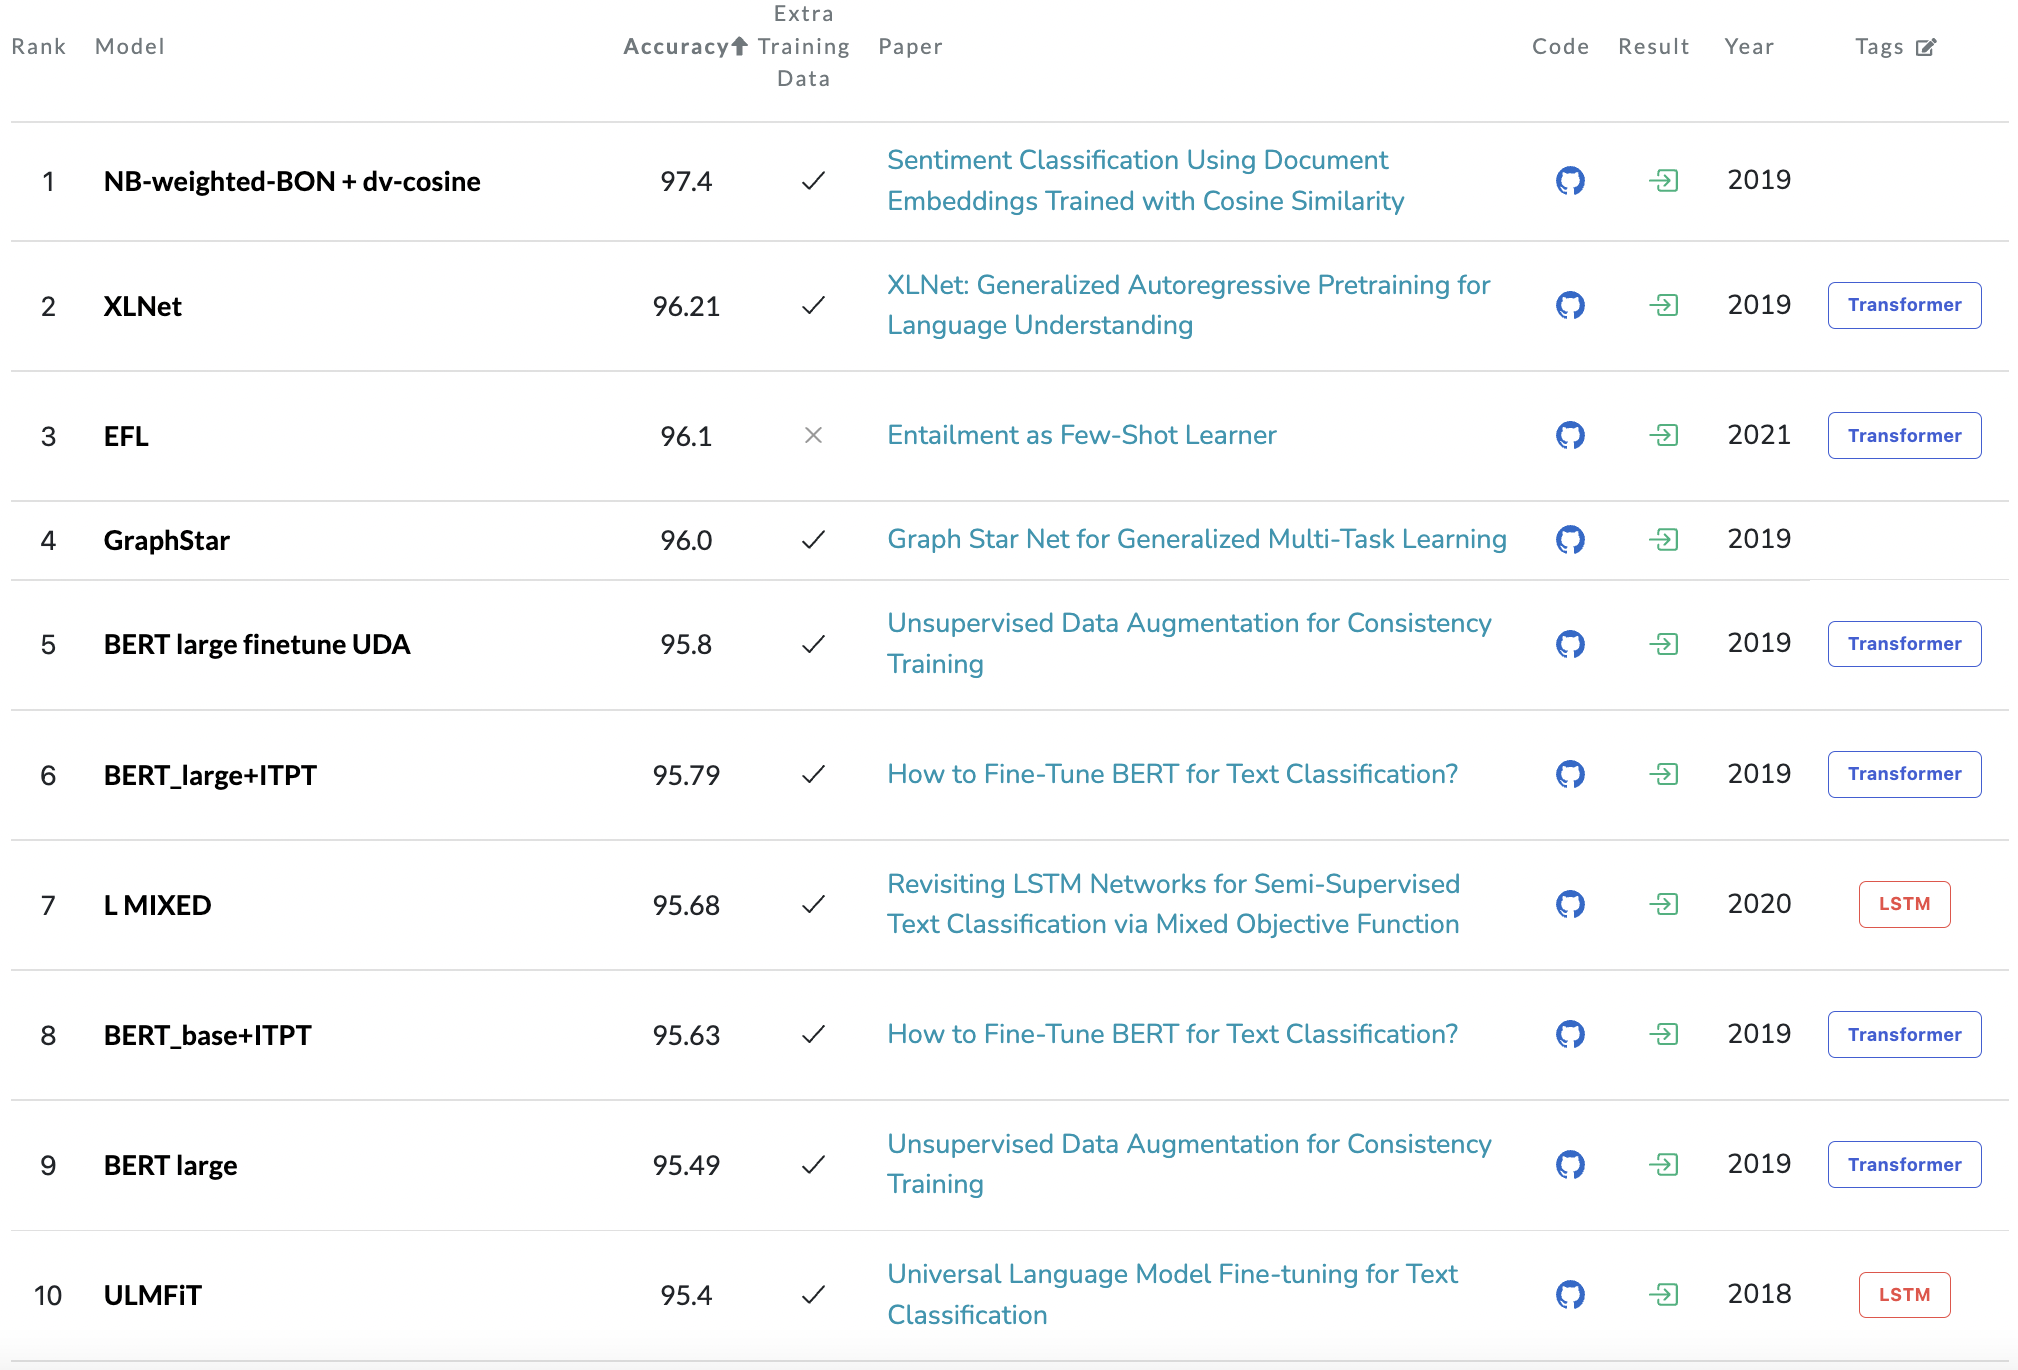
\includegraphics[scale=0.4]{figuras/as-eda-pwc-table.png}
    % \caption[Así aparece el rótulo en el índice]{Así aparece el rótulo en el texto.}
    \caption[Análisis de Sentimiento - Papers with code - Top 10]{\textbf{Esta imagen muestra el ranking de modelos organizados por el accuracy obtenido en el problema de análisis de sentimiento sobre el dataset de reseñas de IMDB. En este ranking podemos ver 7 modelos basados en transformers y la mitad de los modelos en el top 10 son modelos basados en BERT. Fuente: \url{https://paperswithcode.com/sota/sentiment-analysis-on-imdb}}}
    \label{fig-as-eda-pwc-table}
\end{figure}

%%%%%%%%%%%%%%%%%%%%%%%%%%%%%%%%%%%%%%%%%%%%%%%%%%%%%%%%%%%%%%%%%%%%%%%%%%%%%%%%%%%%%%%%%%%%%%%%%%%%%%%%%%%%%%%

\subsection{Arquitectura de la solución}
\label{subsection-as-arquitectura-de-la-solucion}
Como se mencionó anteriormente en la sección \ref{subsection-arquitectura-bert}, la arquitectura de BERT ha sido diseñada para adaptarse a la resolución de distintos problemas a través de un leve ajuste. Este caso en particular se trata de un problema de clasificación de una frase en dos clases objetivos, en otras palabras, dada una frase clasificarla como sentimiento positivo o sentimiento negativo.

La forma de afrontar un problema de clasificación con BERT es en base al token especial [CLS]. Como indican los autores en el \textit{paper} de BERT, ``El primer token de cada secuencia es siempre un token de clasificación especial [CLS]. El estado oculto final correspondiente a este token se utiliza como representación de secuencia agregada para tareas de clasificación."  (\cite{https://doi.org/10.48550/arxiv.1810.04805})

En la imagen \ref{fig-bert-as-architecture} se describe la arquitectura general de la solución propuesta para este problema, donde podemos observar las 12 capas de Transformer que componen el modelo. Cada una de estas capas toma un \textit{embedding} de tokens como entrada y produce la misma cantidad de \textit{embeddings} en la salida. En la salida del último Transformer se construye un clasificador a través del primer \textit{embedding} correspondiente al token [CLS].

\begin{figure}[ht!]
    \centering
    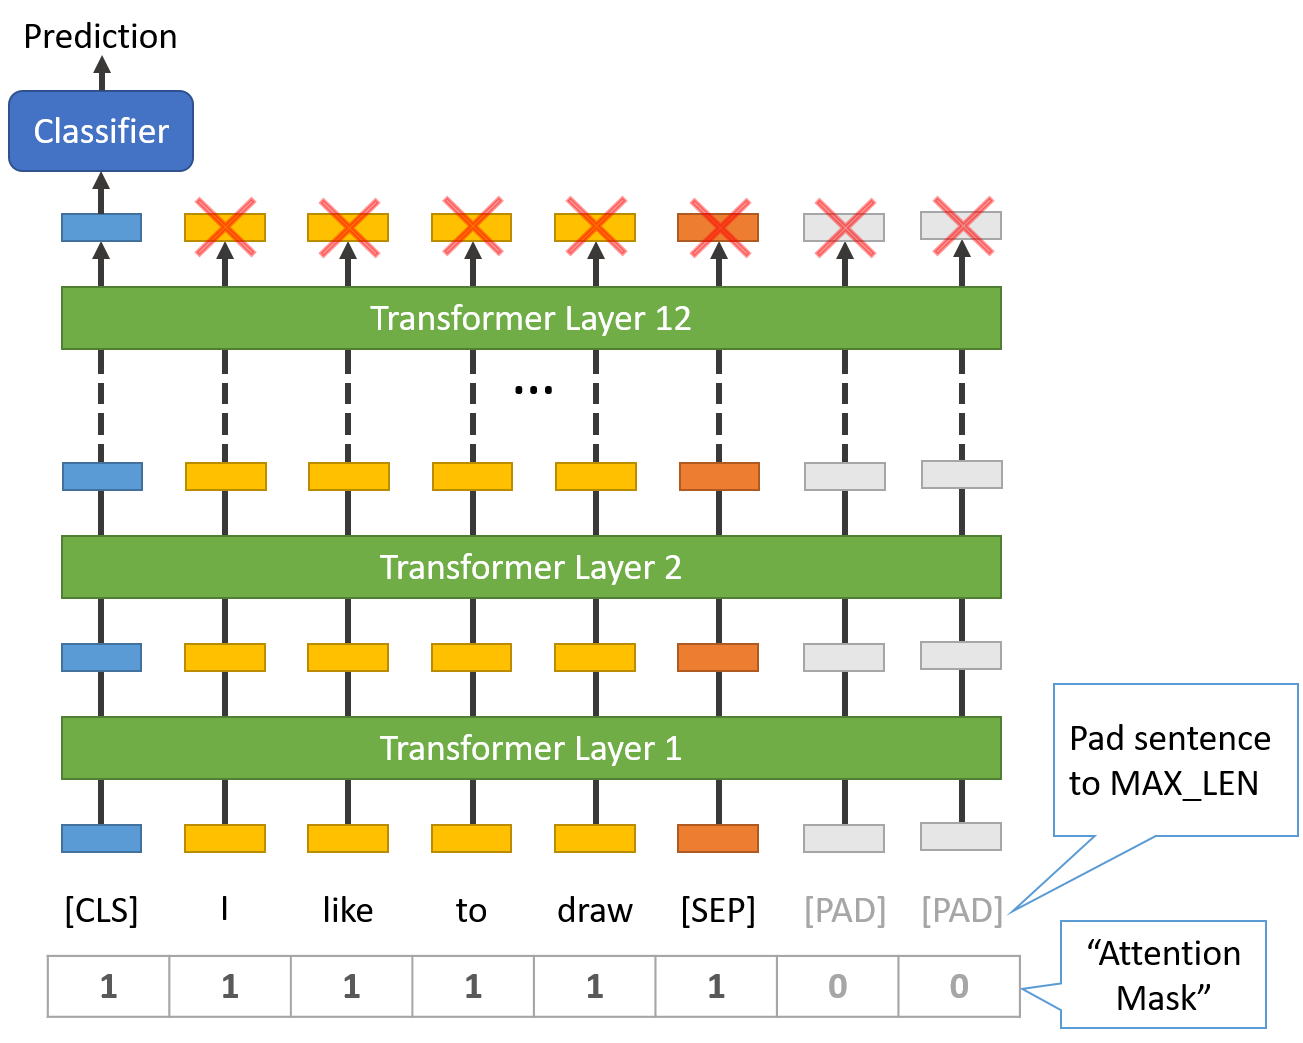
\includegraphics[scale=0.5]{figuras/bert-as-architecture.png}
    % \caption[Así aparece el rótulo en el índice]{Así aparece el rótulo en el texto.}
    \caption[Análisis de Sentimiento - Arquitectura de la solución]{\textbf{Adecuación de la arquitectura de BERT para la solución de problemas de clasificación basados en una frase de entrada. Fuente: \cite{chris_mccormick_and_nick_ryan_bert_2019}}}
    \label{fig-bert-as-architecture}
\end{figure}

%%%%%%%%%%%%%%%%%%%%%%%%%%%%%%%%%%%%%%%%%%%%%%%%%%%%%%%%%%%%%%%%%%%%%%%%%%%%%%%%%%%%%%%%%%%%%%%%%%%%%%%%%%%%%%%

\subsection{Preparación de los datos}
\label{as-preparacion-de-los-datos}

Durante el proceso de preparación de los datos se abordaron dos etapas. La primera de ellas de exploración y saneamiento de los datos. Durante esta primera etapa:

\begin{itemize}
    \item Se identificó y valido que tal como indica la documentación \cite{maas-EtAl:2011:ACL-HLT2011}, el dataset está compuesto por 50000 registros bien balanceados (25000 datos etiquetados como positivos y 25000 datos etiquetados como negativos) como se pudo confirmar una vez fueron cargados los datos. 
    \item Se pudo notar que ciertos registros se encontraban duplicados. Estos registros duplicados fueron removidos.
    \item Se creó y aplicó una función de limpieza que permite para cada una de las reseñas limpiar algunos elementos que podrían causar ruido y carecen de valor en el análisis y entrenamiento del modelo como las etiquetas \acrshort{acr_html}, texto entre corchetes y algunos signos de puntuación.
\end{itemize}

La segunda etapa se basó en un proceso de normalización de los datos de entrada para BERT. Al tratarse BERT de un modelo preentrenado, este espera que los datos de entrada tengan un formato especifico, tal como se indica en la sección \ref{subsection-bert-finetunning}. La normalización de los datos de entrada se basa en la construcción adecuada de los \textit{embeddings} para que el modelo pueda entender cada una de las sentencias de entrada, esto consiste en:

\begin{enumerate}
    \item Como se describe en la arquitectura de la solución (ver figura \ref{fig-bert-as-architecture}), el modelo de BERT tiene dos restricciones:
    \begin{enumerate}
    \item Todas las sentencias de entrada deben tener la misma longitud, por ese motivo las sentencias son truncadas o rellenadas con un token especial denominado [PAD]
    \item La longitud máxima de la sentencia de entrada es de 512 tokens.
    \end{enumerate}
    Al tener sentencias de entrada de longitud variable se optó en este caso por truncar los datos de entrada a una longitud máxima de 512 tokens. En otras palabras estamos basando el entrenamiento en los primeros 512 tokens de cada reseña, desechando el resto de la información. 
    \item Añadir sentencias de entrada que tengan agregados los tokens especiales al comienzo y al final de cada sentencia.
    \begin{enumerate}
    \item El token [SEP] es un token especial que se utiliza para demarcar el fin de una sentencia o la separación entre dos sentencias. En este caso se utiliza como delimitador final de la única sentencia de entrada.
    \item El token [CLS] se debe anteponer a cada sentencia de entrada. Este token es usado en las tareas de clasificación, pero indistintamente del problema a resolver el modelo BERT siempre espera recibirlo como el comienzo de la entrada. La importancia de este token radica en que actúa como una representación agregada para las atareas de clasificación. La última capa oculta de este token se usa como una representación de la sentencia para la clasificación de secuencias.
    \end{enumerate}
    \item Agregar dos embeddings de información para el modelo:
    Al embedding de tokens producto del tokenizador de BERT (Token IDs), se deben agregar dos \textit{embeddings} adicionales:
    \begin{enumerate}
    \item Mask IDs o máscara de atención que diferencia cuales elementos de la secuencia son tokens y cuales son tokens de relleno o padding. Se trata simplemente una matriz de 1s y 0s que indica qué tokens están rellenando y cuáles no. Esta máscara le dice al mecanismo de auto-atención en BERT que no incorpore estos tokens [PAD] en su interpretación de la sentencia.
    \item Segment IDs usado para distinguir diferentes sentencias. En este caso en el que tenemos una sola sentencia se trata de un vector de 0s.
    \end{enumerate}
\end{enumerate}

Adicionalmente es importante mencionar que existen técnicas y trabajos enfocados en cómo manejar la limitación que presenta BERT en cuanto a la extinción de los tokens de la secuencia de entrada. 

Existen tres enfoques distintos basados en el costo computacional:
\begin{itemize}
    \item \textbf{Bajo costo computacional:} Seleccionar una parte del texto original. Los ejemplos incluyen elegir los primeros n tokens, los últimos n tokens o compilar una nueva instancia de texto a partir del principio y el final de la instancia de texto original.
    \item \textbf{Costo computacional medio a alto:} Usar modelos de Transformers recientes (como Longformer) que tienen un límite de 4096 tokens en lugar de 512. Estos nuevos métodos tienen mecanismos de atención modificados que reducen el costo computacional.
    \item \textbf{Alto costo computacional:} Dividir la instancia de texto en fragmentos que se ajusten a un modelo como BERT con un límite estándar de 512 tokens por instancia e implementar el modelo en cada parte por separado, luego unir las representaciones vectoriales resultantes.
\end{itemize}

En el artículo de \cite{Fiok_2021_TextGuideLong} además de proponer un nuevo método llamado Text Guide, que es un método de bajo coste computacional el cual pretende hacer un truncamiento mas inteligente de la instancia de entrada.

Por último mencionar que \cite{FTBERTCLAS_https://doi.org/10.48550/arxiv.1905.05583} en su \textit{paper} hace una comparación usando distintas técnicas para truncar el texto, tomando en algunos casos el principio, en otros casos el final y en algunos casos haciendo combinaciones de distintos segmentos del texto. De este trabajo igual podemos concluir que la diferencia del performance del modelo no es significativa entre las distintas técnicas. 

Por las razones antes expuestas y entendiendo que el m´todo elegido no impactará mucho el performance del modelo,  para este trabajo se decidió utilizar un truncamiento simple tomando los primeros 512 tokens de la sentencia de entrada.


%%%%%%%%%%%%%%%%%%%%%%%%%%%%%%%%%%%%%%%%%%%%%%%%%%%%%%%%%%%%%%%%%%%%%%%%%%%%%%%%%%%%%%%%%%%%%%%%%%%%%%%%%%%%%%%

\subsection{Modelo y Fine Tuning}
\label{as-finetunning}

El modelo de BERT se obtuvo desde Tensorflow Hub (\url{https://www.tensorflow.org/hub}). TensorFlow Hub es un repositorio de modelos de aprendizaje automático preentrenados, listos para poder implementar un fine-tunning.

Se usó como modelo BERT preentrenado la versión bert\_multi\_cased\_L-12\_H-768\_A-12. Para hacer el clasificador se optó por usar el API Keras de Tensorflow tomando las salidas del modelo de BERT, específicamente el pooled\_output (embedding del token [CLS]) y creando una capa única para la tarea de clasificación, para ayudar a prevenir el sobreajuste se hizo un droput de 10\%. En esta última capa, se aplica la función softmax para obtener las probabilidades predichas del modelo entrenado.

Para entrenar el modelo propuesto se utilizo como valores de los hiperparámetros los recomendados en el \textit{paper} de BERT. Según los autores del \textit{paper} BERT no necesita muchas epocas para ser entrenado y recomiendan que sean entre 2 y 4. \cite{https://doi.org/10.48550/arxiv.1810.04805}:

\begin{itemize}
    \item Tamaño del lote = 8
    \item Tasa de aprendizaje = 2e-5
    \item Longitud máxima de secuencia = 512
    \item Épocas = 3
\end{itemize}

\begin{figure}[ht!]
    \centering
    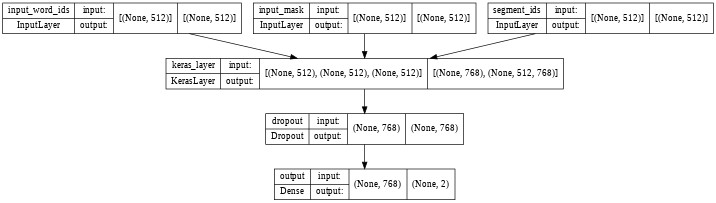
\includegraphics[scale=0.6]{figuras/as-modelo.png}
    % \caption[Así aparece el rótulo en el índice]{Así aparece el rótulo en el texto.}
    \caption[Análisis de Sentimiento - Modelo de la solución]{\textbf{Modelo de BERT propuesto para la solución de este problema de clasificación. En el modelo se observan como entrada las tres embeddings que la conforman, el token embedding, el de segmentación y el posicional, estos van directamente a la capa preentrenada de BERT, luego se agrega una capa de dropout y una última capa que recibe el dropout del embedding del token [CLS] y como salida tiene solo dos neuronas, una para cada clase a predecir. Fuente: Imagen propia}}
    \label{fig-as-modelo}
\end{figure}

El entrenamiento se realizó usando Google Colab y utilizando la GPU (Graphic Processing Unit). La duración del entrenamiento ha sido:

\begin{itemize}
    \item Primera Época = 3368 segundos.
    \item Segunda Época = 3373 segundos. 
    \item Tercera Época = 3372 segundos.
    \item Entrenamiento total = 10113 segundos, aproximadamente 2 horas y 50 minutos.
\end{itemize}

El código fuente del entrenamiento se encuentra en el repositorio Github \url{https://github.com/lsizaguirre/09MIAR-TFM}

%%%%%%%%%%%%%%%%%%%%%%%%%%%%%%%%%%%%%%%%%%%%%%%%%%%%%%%%%%%%%%%%%%%%%%%%%%%%%%%%%%%%%%%%%%%%%%%%%%%%%%%%%%%%%%%

\subsection{Resultados y Conclusiones.}
\label{as-resultados-y-conclusiones}

Podemos observar que con una configuración de red muy sencilla y con los parámetros recomendados para el fine-tunning se obtienen resultados bastante buenos y cercanos a los que definen el estado del arte. Se podría intentar hacer un ajuste más sofisticado y con ello obtener mejores resultados.

Las siguientes imágenes muestran algunas de las métricas obtenidas durante la evaluación del experimento.

\begin{figure}[ht!]
    \centering
    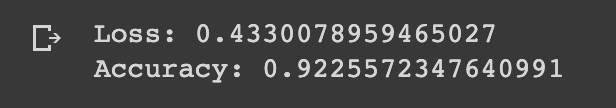
\includegraphics[scale=0.6]{figuras/as-resultados-1.png}
    % \caption[Así aparece el rótulo en el índice]{Así aparece el rótulo en el texto.}
    \caption[Análisis de Sentimiento - Resultados - Accuracy y Loss]{\textbf{Accuracy y Loss obtenidos con el modelo. Fuente: Imagen propia}}
    \label{fig-as-resultados-1}
\end{figure}

\begin{figure}[ht!]
    \centering
    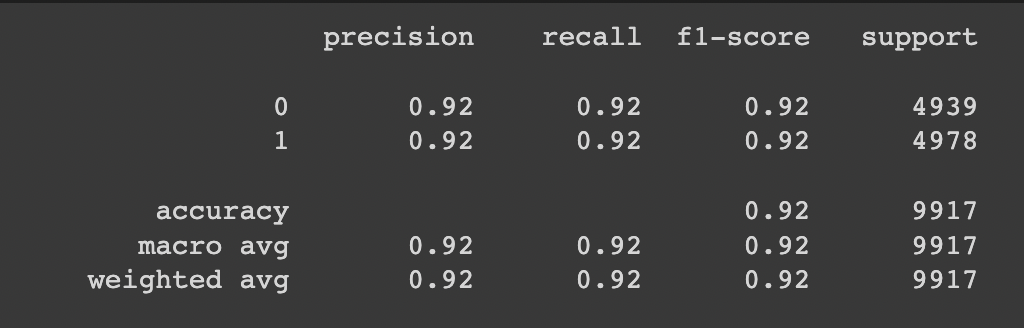
\includegraphics[scale=0.6]{figuras/as-resultados-2.png}
    % \caption[Así aparece el rótulo en el índice]{Así aparece el rótulo en el texto.}
    \caption[Análisis de Sentimiento - Resultados - Métricas de clasificación]{\textbf{Métricas de clasificación obtenidas en el modelo. Fuente: Imagen propia}}
    \label{fig-as-resultados-2}
\end{figure}

\begin{figure}[ht!]
    \centering
    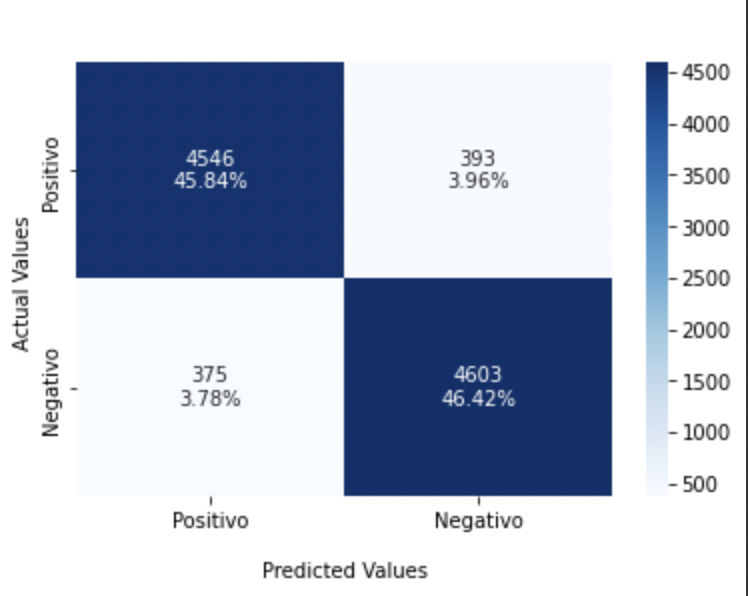
\includegraphics[scale=0.6]{figuras/as-resultados-3.png}
    % \caption[Así aparece el rótulo en el índice]{Así aparece el rótulo en el texto.}
    \caption[Análisis de Sentimiento - Resultados - Matriz de confusión]{\textbf{Matriz de confusión resultado de la evaluación del modelo. Fuente: Imagen propia}}
    \label{fig-as-resultados-3}
\end{figure}


\clearpage 
%%%%%%%%%%%%%%%%%%%%%%%%%%%%%%%%%%%%
% SECTION - PREGUNTAS Y RESPUESTAS 
%%%%%%%%%%%%%%%%%%%%%%%%%%%%%%%%%%%%

\section{Problema de Respuesta a Preguntas}
\label{section-preguntas-y-respuestas}

%%%%%%%%%%%%%%%%%%%%%%%%%%%%%%%%%%%%%%%%%%%%%%%%%%%%%%%%%%%%%%%%%%%%%%%%%%%%%%%%%%%%%%%%%%%%%%%%%%%%%%%%%%%%%%%

\subsection{Descripción del problema}
\label{subsection-qa-descripcion-problema}

Vivimos en una época donde la actividad digital forma parte de nuestro día a día. Todos los días generamos una cantidad enorme de datos e información, interactuando a través de redes sociales, trabajando conectados a Internet, etc. A medida que aumenta la información, se vuelve más difícil recuperar una pieza de información relevante de manera eficiente. En este sentido, la tarea de Respuesta a Preguntas o \textit{Question Answering} (QA, por sus siglas en inglés) es un campo de la ciencia de la computación y el NLP que tiene como objetivo crear sistemas que puedan responder de forma automática preguntas en lenguaje natural.  

Los sistemas QA intentan encontrar automáticamente la respuesta contextual y semánticamente correcta para una pregunta proporcionada en un texto. En general, los tres componentes asociados con los sistemas QA son:

\begin{enumerate}
    \item Clasificación de preguntas
    \item Recuperación de información
    \item Extracción/generación de respuestas
\end{enumerate}

En este trabajo se usará BERT como modelo base para resolver este problema. La idea en este caso es que se le dará un párrafo al modelo de BERT que contendrá información acerca de un tema, y vamos a buscar respuestas con respecto a preguntas relacionadas con ese tema. Para ello, se generarán preguntas cuyas respuestas se encuentren dentro de los textos del párrafo.

%%%%%%%%%%%%%%%%%%%%%%%%%%%%%%%%%%%%%%%%%%%%%%%%%%%%%%%%%%%%%%%%%%%%%%%%%%%%%%%%%%%%%%%%%%%%%%%%%%%%%%%%%%%%%%%

\subsection{Selección del Dataset}
\label{subsection-qa-dataset-imdb}

Para este experimento se usó \textbf{\acrfull{acr_squad}}. Este es un conjunto de datos de respuesta a preguntas publicado en el año 2016 por investigadores de la Universidad de Stanford, junto al \textit{paper} ``\textit{SQuAD: 100000+ Questions for Machine Comprehension of Text}'' \citep{SQUADv1_https://doi.org/10.48550/arxiv.1606.05250}

Existe una segunda versión de SQuAD (v2.0) publicada por los mismos investigadores en el año 2018 en el \textit{paper} ``\textit{Know What You Don't Know: Unanswerable Questions for SQuAD}'' \citep{SQUADv2_https://doi.org/10.48550/arxiv.1806.03822}. Esta versión se diferencia de la primera en que en algunas oportunidades la respuesta no se encuentra en el texto original y está enfocada a ser utilizada en soluciones donde el modelo debe fabricar la respuesta de algún modo. Por simplicidad en este trabajó se utilizó la versión 1.1 de este conjunto de datos.

Este conjunto de datos contiene un total de 107785 preguntas extraídas de un conjunto de 536 artículos seleccionados de la Wikipedia, en un amplio rango de tópicos. Los autores del \textit{paper} mencionan que este conjunto de datos se diferencia a los que se habían publicado con anterioridad en que las respuestas son de formato libre y no están acotadas a un conjunto de opciones lo que hace el problema más interpretativo y con una cantidad bastante grande de opciones. 

Otro aspecto relevante es que los archivos que componen este conjunto de datos se encuentran en \textit{formato .json} y vienen en las siguientes particiones, generadas aleatoriamente:

\begin{itemize}
    \item \textbf{train-v1.1.json:} Es un \gls{gls_json} que contiene el 80\% de los datos y contiene el conjunto de entrenamiento o training set. Es el subconjunto del dataset donde están almacenadas las secuencias que se utilizarán para hacer el entrenamiento.
    \item \textbf{dev-v1.1.json:} Es un \gls{gls_json} que contiene el 10\% de los datos y contiene el conjunto de validación o validation test. Es el subconjunto de datos que se utilizarán para hacer la evaluación.
    \item El 10\% restante de registros son usados para la validación final usada en el benchmark y este conjunto de datos no lo hacen disponible. testing set.
\end{itemize}

%%%%%%%%%%%%%%%%%%%%%%%%%%%%%%%%%%%%%%%%%%%%%%%%%%%%%%%%%%%%%%%%%%%%%%%%%%%%%%%%%%%%%%%%%%%%%%%%%%%%%%%%%%%%%%%

\subsection{Estado del arte}
\label{subsection-qa-estado-del-arte}

Hay dos métricas dominantes utilizadas por muchos conjuntos de datos de respuesta a preguntas, incluido SQuAD: la coincidencia exacta (EM) y puntaje F1. Estos puntajes se calculan en pares individuales de pregunta y respuesta. Cuando son posibles varias respuestas correctas para una pregunta determinada, se calcula la puntuación máxima sobre todas las posibles respuestas correctas. Las puntuaciones generales de EM y F1 se calculan para un modelo promediando las puntuaciones de los ejemplos individuales.

\begin{itemize}
    \item \textbf{Coincidencia exacta o Exact Match (EM, por sus siglas en inglés):} esta métrica es tan simple como parece. Para cada par de pregunta y respuesta, si los caracteres de la predicción del modelo coinciden exactamente con los caracteres de (una de) las respuestas verdaderas, EM = 1; de lo contrario, EM = 0. Esta es una métrica estricta de todo o nada, estar equivocado por un solo carácter da como resultado una puntuación de 0. Al evaluar contra un ejemplo negativo, si el modelo predice cualquier texto, automáticamente recibe un 0 para ese ejemplo.
    \item \textbf{La puntuación F1 o F1 score (en inglés):} es una métrica común para los problemas de clasificación y se usa ampliamente en la tarea de QA. Es apropiado cuando nos preocupamos por igual por la precisión y la memoria. En este caso, se calcula sobre las palabras individuales de la predicción frente a las de la respuesta verdadera. La cantidad de palabras compartidas entre la predicción y la verdad es la base de la puntuación F1: la precisión es la relación entre la cantidad de palabras compartidas y la cantidad total de palabras en la predicción, y el recuerdo o memoria es la relación entre la cantidad de palabras compartidas. al número total de palabras en la verdad fundamental.
\end{itemize}

Es indudable que BERT ha provocado un avance considerable en el estado del arte de varias tareas de NLP. Específicamente en la tarea de QA podemos ver tanto en el leaderboard  de SQuAD como en el de otros conjuntos de datos similares como CoQA \citep{CoQA_https://doi.org/10.48550/arxiv.1808.07042} que la mayoría de modelos que lideran están basados en BERT.

\begin{figure}[ht!]
    \centering
    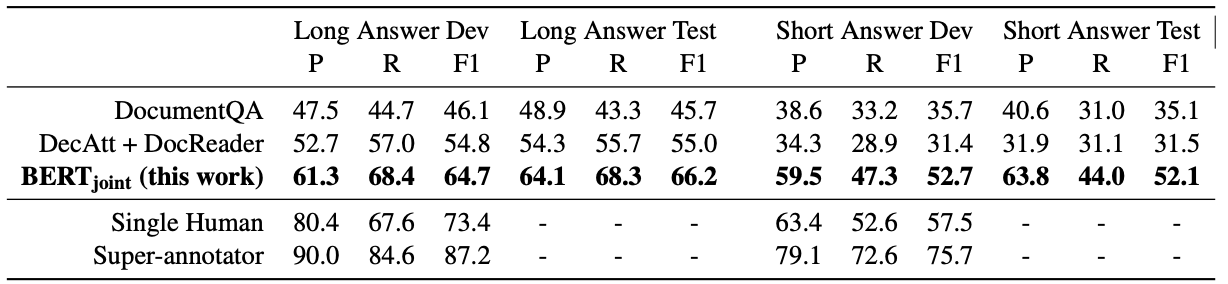
\includegraphics[scale=0.69]{figuras/qa-eda-vshuman.png}
    % \caption[Así aparece el rótulo en el índice]{Así aparece el rótulo en el texto.}
    \caption[Preguntas y Respuestas - Comparación rendimiento BERT vs humanos]{\textbf{En este estudio \cite{BERT_baseline_for_NQ_https://doi.org/10.48550/arxiv.1901.08634} comparan el desempeño de BERT contra un humano común y un humano experto. Se evidencia el mejor desempeño de BERT en ciertos casos. Fuente: \cite{BERT_baseline_for_NQ_https://doi.org/10.48550/arxiv.1901.08634}}}
    \label{fig-qa-eda-vshuman}
\end{figure}

Para evaluar el estado del arte relacionado a la solución de preguntas y respuestas sobre el dataset SQuAD en su versión 1.0 se utilizaron diversas fuentes. 

En el \textit{paper} realizado por \citet{BERT_baseline_for_NQ_https://doi.org/10.48550/arxiv.1901.08634} titulado ``\textit{A BERT Baseline for the Natural Questions}'' los autores concluyen que BERT debe ser la nueva línea base y que constituye un buen punto de partida para los modelos de preguntas y respuestas y \textit{datasets} con características similares. En este mismo estudio los autores comparan el desempeño de BERT con otros modelos que resolvían la tarea en ese momento y además lo compararon con el desempeño de la tarea realizada por un humano común y un humano experto. (ver figura \ref{fig-qa-eda-vshuman}). Los autores concluyen que los resultados obtenidos por los modelos de respuesta a preguntas basados en BERT también se están acercando rápidamente al rendimiento humano informado para estos conjuntos de datos.

Existen otros estudios, como el presentado en el \textit{paper} ``\textit{Comparative Study of Machine Learning Models and BERT on SQuAD}'' de \cite{SQuAD_Comparison_https://doi.org/10.48550/arxiv.2005.11313} donde realizan un análisis comparativo del rendimiento de ciertos modelos populares en el aprendizaje automático y el modelo de BERT sobre SQuAD, brindando BERT una mayor precisión que otros modelos.

En el ranking de la página oficial de SQuAD (\url{https://rajpurkar.github.io/SQuAD-explorer/}) podemos observar muchos modelos basados en ALBERT \cite{ALBERT_https://doi.org/10.48550/arxiv.1909.11942}. ALBERT es una versión de BERT mucho más ligera con 12 millones de parámetros en vez de 110 millones como los que contiene BERT. En el \textit{paper} original de ALBERT llamado ``\textit{ALBERT: A Lite BERT for Self-supervised Learning of Language Representations}''  comparan el desempeño de ALBERT con BERT en las tareas de SQuAD obteniendo resultados bastante similares (ver figura \ref{fig-qa-eda-albert})

\begin{figure}[ht!]
    \centering
    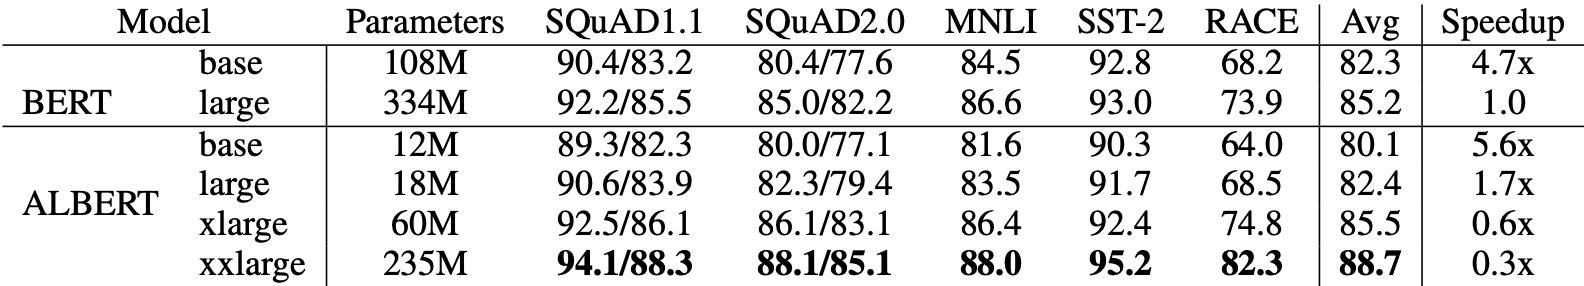
\includegraphics[scale=0.5]{figuras/qa-eda-albert.png}
    % \caption[Así aparece el rótulo en el índice]{Así aparece el rótulo en el texto.}
    \caption[Preguntas y Respuestas - Comparación BERT vs humanos]{\textbf{Comparación de los resultados obtenidos en distintas tareas de NLP entre BERT y su variante ALBERT. Para las tareas SQuAD los dos números equivalen a F1 y EM. Fuente: \cite{ALBERT_https://doi.org/10.48550/arxiv.1909.11942}}}
    \label{fig-qa-eda-albert}
\end{figure}

%%%%%%%%%%%%%%%%%%%%%%%%%%%%%%%%%%%%%%%%%%%%%%%%%%%%%%%%%%%%%%%%%%%%%%%%%%%%%%%%%%%%%%%%%%%%%%%%%%%%%%%%%%%%%%%

\subsection{Arquitectura de la solución}
\label{subsection-qa-arquitectura-de-la-solucion}

Como ya se mencionó en la sección \ref{subsection-arquitectura-bert}, la arquitectura de BERT ha sido diseñada para adaptarse a la resolución de distintos problemas a través de un leve ajuste, por este motivo es que en BERT tenemos dos formas diferentes de manejar la entrada y la salida del modelo. 

Con respecto a la entrada, una de las formas es cuando se tiene un vector que se supone representa toda una frase en su completitud y es básicamente la forma que se utiliza en las tareas de clasificación. La segunda forma de entrada es una lista de vectores, cada uno de los cuales es una representación de las palabras en el contexto que las rodea. Esta segunda forma de entrada es particularmente la que se utiliza en este tipo de problemas al no tratarse de un problema de clasificación como en el experimento anterior.

Como entrada se definieron dos frases, la primera frase representa el texto en el que hay que buscar la información. La segunda frase representa la pregunta que se quiere resolver. En la primera frase, lo que se necesita es buscar dónde empieza y dónde termina la hipotética respuesta a nivel de tokens y ese nivel de tokens luego es traducido a nivel de palabras. De esa forma se busca la respuesta dentro de la primera oración.

Con respecto a la salida, para este caso no se usa el \textit{Pooled Output}, el cual es una representación del token de clasificación [CLS], un embedding de toda la frase. Por el contrario, se usa el \textit{Sequence Output}, el cual está representado por una lista de vectores (embedding), uno para cada una de las palabras, de esta forma se podrá localizar las más probables de ser la el inicio y el final de la respuesta.

Casi siempre que se utiliza BERT para generar la solución de una tarea, lo único que hay que hacer es añadir una capa densa al final antes de hacer ningún ajuste de los parámetros. Estas capas densas se le aplica a cada uno de los elementos, a cada vector y nos va a dar dos posibles respuestas, dos neuronas en la capa de salida.

La primera nos representará una puntuación de qué tan probable es que esa palabra sea la posición inicial en la que empieza la respuesta y la segunda neurona representará una puntuación de qué tan probable es que esa palabra sea la la que finaliza la respuesta De esa forma, simplemente aplicando una capa densa con dos neuronas a cada vector, a cada representación vectorial de las palabras, obtendremos un puntaje de qué tan susceptible es de ser la palabra que inicia o que finaliza la respuesta a la pregunta que estamos buscando.

Finalmente se debe construir un par de listas de todos los puntajes de qué tan probable es que sean el inicio o el final de la respuesta para cada una de las palabras. Una lista para el inicio y otro para el final. La respuesta será la frase o secuencia de palabras contenidas entre el token que tenga el mayor puntaje o probabilidad de ser el inicio de la respuesta y el token con mayor puntaje de ser el final de la respuesta.

Como el proceso de tokenización de BERT tiende a romper palabras, estas se tendrán que reconstruir correctamente.

\begin{figure}[ht!]
    \centering
    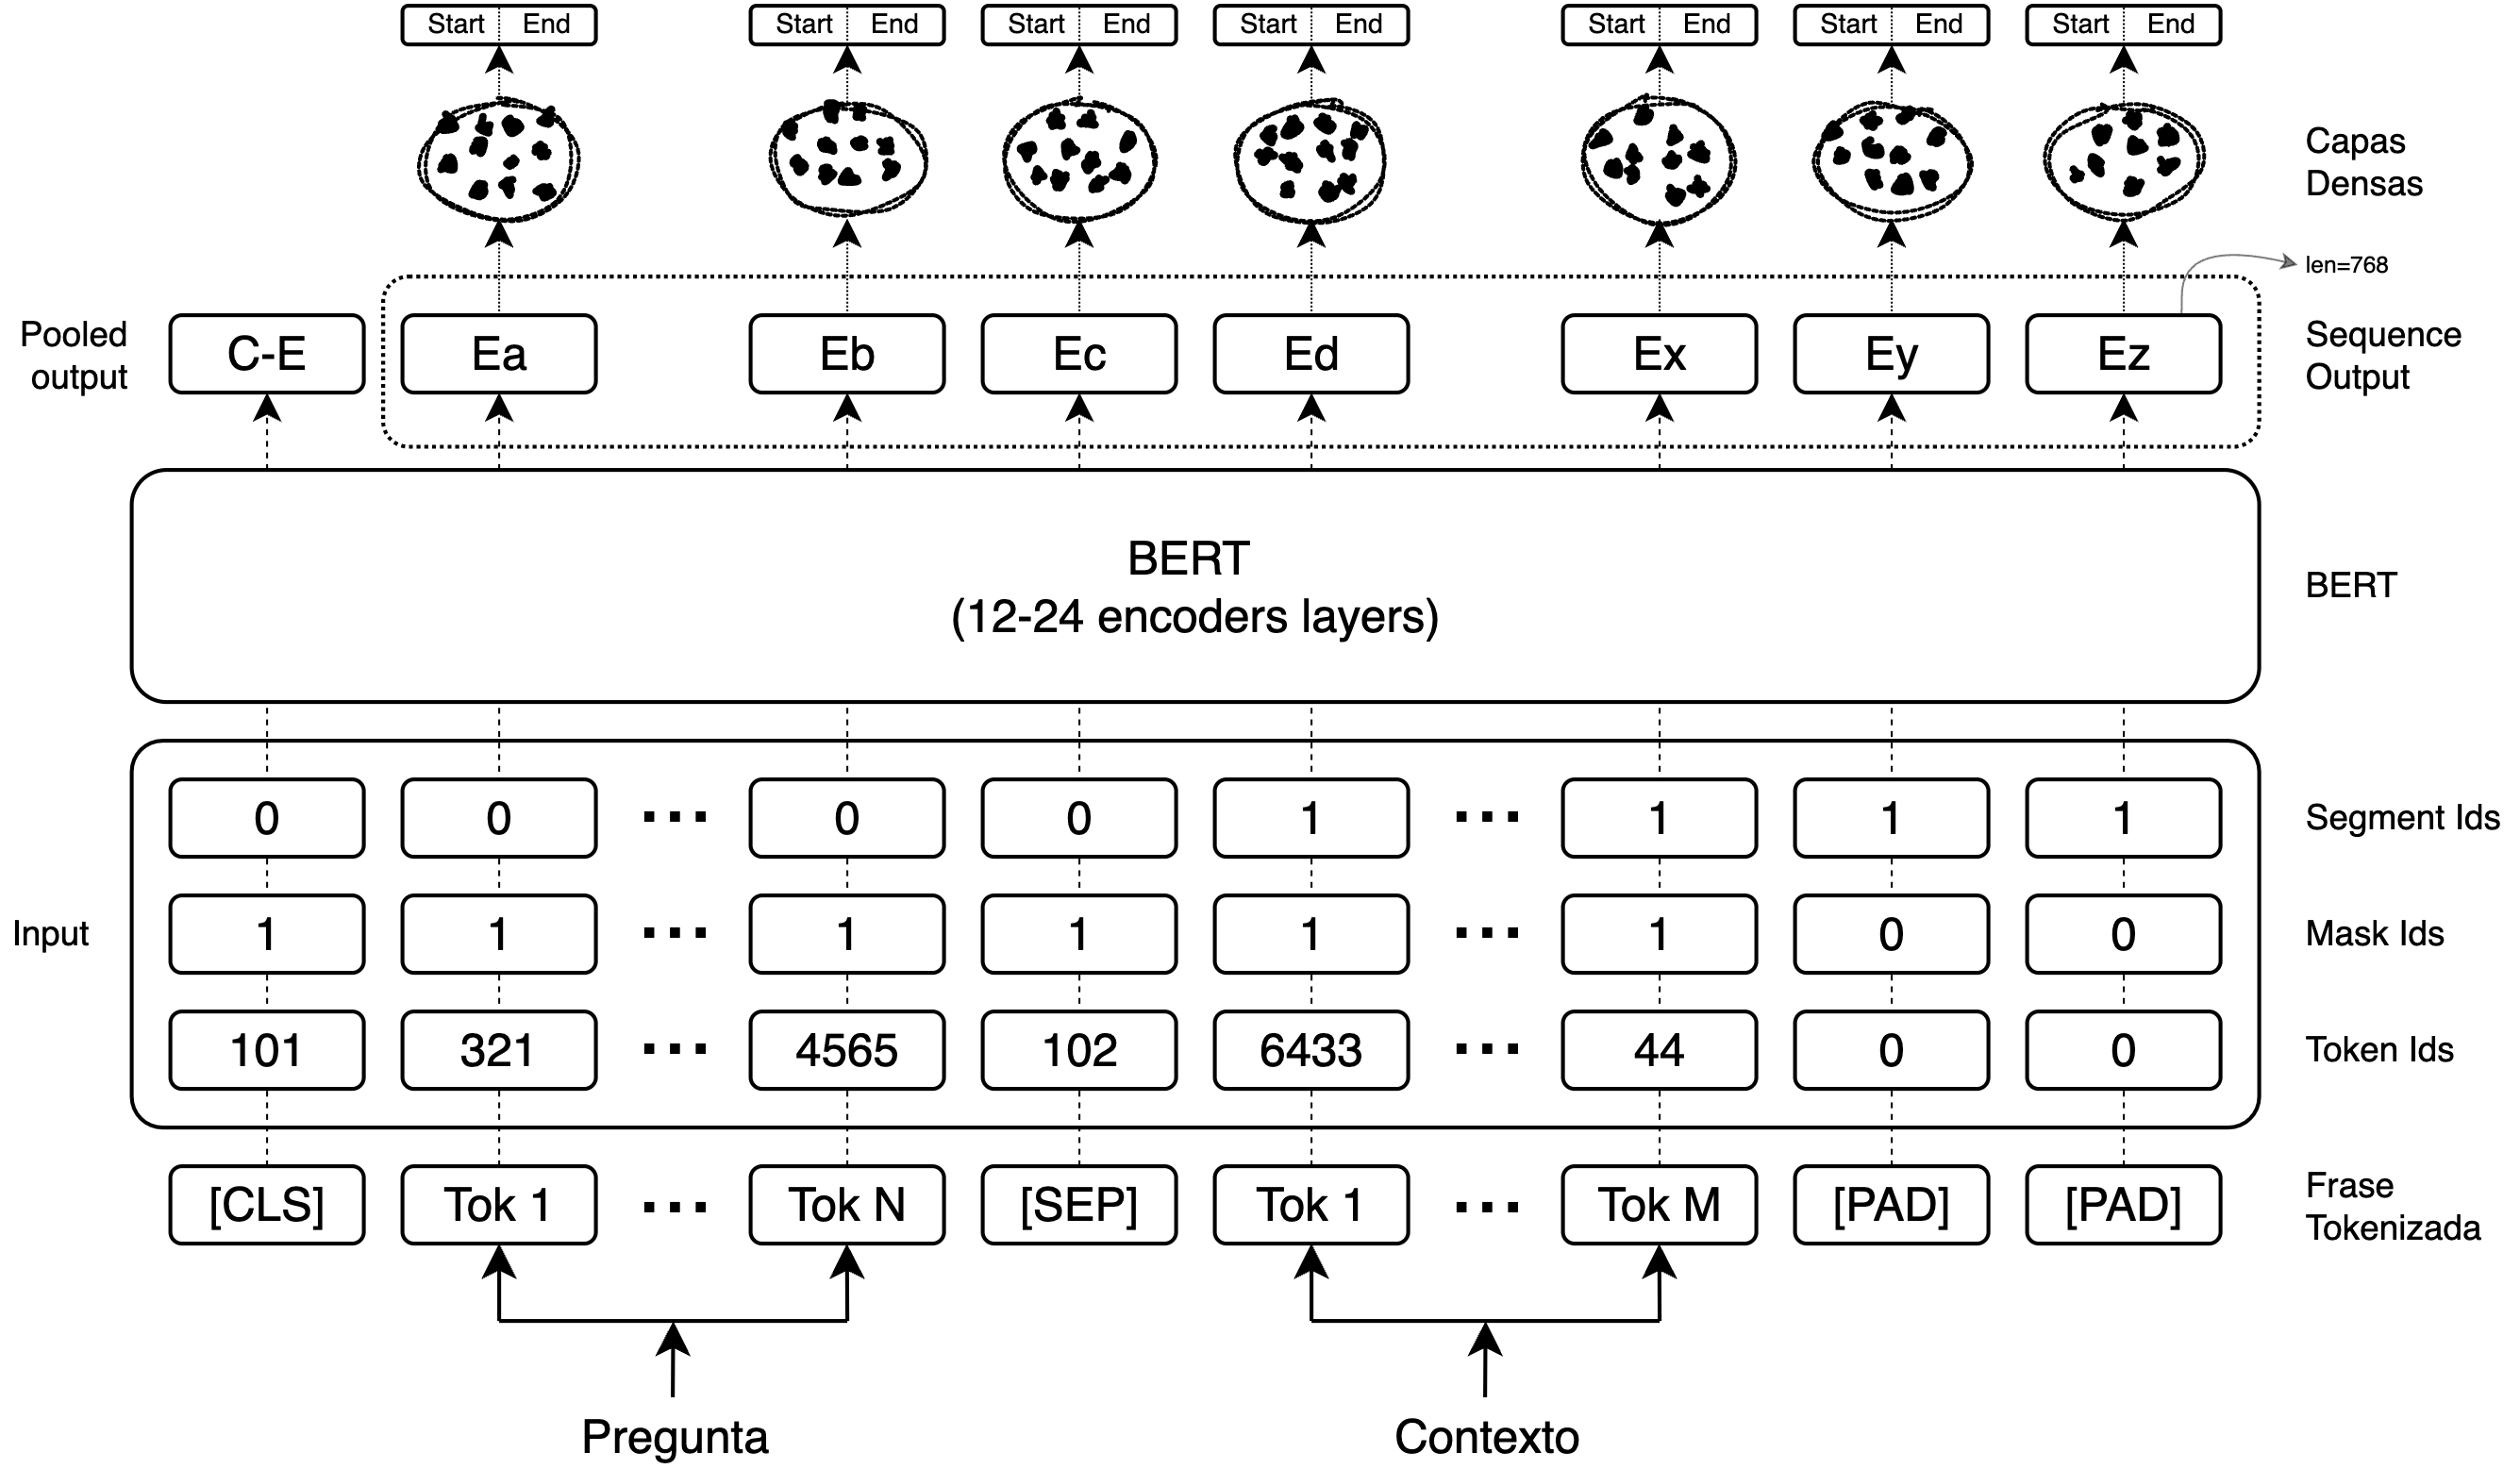
\includegraphics[scale=0.155]{figuras/bert-qa-architecture.png}
    % \caption[Así aparece el rótulo en el índice]{Así aparece el rótulo en el texto.}
    \caption[Preguntas y Respuestas - Arquitectura de la solución]{\textbf{Adecuación de la arquitectura de BERT para la solución de problemas de preguntas y respuestas. Fuente: Imagen propia.}}
    \label{fig-bert-qa-architecture}
\end{figure}

%%%%%%%%%%%%%%%%%%%%%%%%%%%%%%%%%%%%%%%%%%%%%%%%%%%%%%%%%%%%%%%%%%%%%%%%%%%%%%%%%%%%%%%%%%%%%%%%%%%%%%%%%%%%%%%

\subsection{Preparación de los datos}
\label{subsection-qa-preparacion-de-los-datos}

La entrada del modelo BERT para problemas de \textit{question answering} está compuesta por dos frases, la pregunta y el contexto. La forma de manejar la entrada es a través de la estructura mostrada en la figura \ref{fig-bert-qa-architecture}, donde podemos ver:

\begin{enumerate}
    \item Al igual que el experimento anterior y en todos los problemas donde usemos BERT, el token [CLS] se debe anteponer a cada sentencia de entrada. Este token es usado en las tareas de clasificación, pero indistintamente del problema a resolver el modelo BERT siempre espera recibirlo como el comienzo de la entrada.
    \item Seguido al token [CLS] se colocarán los tokens correspondientes a las palabras que componen la pregunta.
    \item A esto le procederá el token especial [SEP] que en este caso tiene un significado distinto dentro de la entrada al experimento anterior. La idea en este caso es que el token [SEP] separará la pregunta del contexto.
    \item En el segment embedding se debe marcar desde el principio de la frase de entrada hasta el token [SEP] como el segmento inicial.
    \item En el resto del token embedding se colocarán los tokens que correspondan al contexto o referencia.
    \item Al igual que en el experimento anterior BERT presenta algunas restricciones con respecto a la entrada:
    \begin{enumerate}
    \item Todas las sentencias de entrada deben tener la misma longitud.
    \item La longitud máxima de la sentencia de entrada es de 384 tokens. Esta longitud es un estándar en el conjunto de datos de SQuAD por dos razones, tener la mayoría de las preguntas y contextos tokenizados sin ningún truncamiento y mantener una longitud limitada para acelerar el entrenamiento.
    \end{enumerate}
\end{enumerate}

A diferencia del problema anterior (ver sección \ref{section-analisis-de-sentimiento}), el conjunto de datos asociado a este problema se encuentra en un \gls{gls_json} que necesita ser preprocesado. Sin embargo, esta tarea de preprocesado de datos es una tarea que se simplifica considerablemente comparado con el proceso del experimento anterior debido a un conjunto de funciones que provee Google para trabajar con el conjunto de datos de SQuAD que ya se encuentran escritas y disponibles en su librería Official.nlp.bert. 

Lo que se logra con estas librerías es transformar los datos de entrenamiento de SQuAD a datos utilizables por las librerías de Tensorflow. Para ello se utilizará la función \textbf{\textit{generate\_tf\_record\_from\_json\_file}}, dejando escrita, su salida, en un
archivo llamado \textbf{\textit{train\_meta\_data}}, divido en cuatro partes. Este archivo ya estará
listo para ser utilizado, también se inicializa el tamaño del batch para el entrenamiento, en este caso será de tamaño 4.

Una vez dado este paso ya se obtienen los datos “tokenizados”, luego a través de la función \textbf{\textit{create\_squad\_dataset}} y a partir de los archivos mencionados con anterioridad, se crea el \textit{dataset} de entrenamiento. De esa forma ya se tendrán listos los datos para entrenar el modelo. 

%%%%%%%%%%%%%%%%%%%%%%%%%%%%%%%%%%%%%%%%%%%%%%%%%%%%%%%%%%%%%%%%%%%%%%%%%%%%%%%%%%%%%%%%%%%%%%%%%%%%%%%%%%%%%%%

\subsection{Modelo y Fine Tuning}
\label{subsection-qa-finetunning}

Al igual que el experimento anterior, el modelo de BERT se obtuvo desde Tensorflow Hub (\url{https://www.tensorflow.org/hub}). Se usó como modelo BERT preentrenado la versión bert\_en\_uncased\_L-12\_H-768\_A-12 al principio se usó la versión bert\_multi\_cased\_L-12\_H-768\_A-12, pensando que se obtendrían mejores resultados usando entradas en distintos idiomas, pero los resultados no fueron buenos. 

Adicionalmente y haciendo uso del API Keras de Tensorflow se creó una ``capa SQuAD'', esta es una capa compuesta por redes neuronales densamente conectadas, la cual será entrenada para devolver dos valores numéricos.

Estos valores representarán dos posiciones en el contexto, que determinarán de dónde se obtendrán el resultado, una vez obtenido el resultado. El resultado calculado se podrá comparar con el resultado esperado y, de esta forma, en base a la evaluación del error cometido, empezar el aprendizaje de las neuronas de la red densamente conectada. 

Como recomienda Tensorflow en su página oficial (\url{https://www.tensorflow.org/text/tutorials/fine_tune_bert}), la función de perdida se implementó a través del método \textbf{\textit{sparse\_categorical\_crossentropy}} de \textbf{\textit{tf.keras.backend}}.

Para entrenar el modelo propuesto se utilizó como valores de los hiperparámetros los recomendados en el \textit{paper} de BERT. Según los autores del \textit{paper} BERT no necesita muchas épocas para ser entrenado y recomiendan que sean entre 2 y 4. \cite{https://doi.org/10.48550/arxiv.1810.04805}:

\begin{itemize}
    \item Tamaño del entrenamiento = 88641 
    \item Número de lotes = 3000 
    \item Tamaño del lote = 4
    \item Tasa de aprendizaje = 2e-5
    \item Longitud máxima de secuencia = 512
    \item Épocas = 3
\end{itemize}

El entrenamiento se realizó usando Google Colab y utilizando la \acrlong{acr_tpu} (\acrshort{acr_tpu}, por sus siglas en inglés). La duración del entrenamiento ha sido:

\begin{itemize}
    \item Primera Época = 12863 segundos.
    \item Segunda Época = 10381 segundos. 
    \item Tercera Época = 11303 segundos.
    \item Entrenamiento total = 34537 segundos, aproximadamente 9 horas y 40 minutos.
\end{itemize}

El código fuente del entrenamiento se encuentra en el repositorio Github \url{https://github.com/lsizaguirre/09MIAR-TFM}

%%%%%%%%%%%%%%%%%%%%%%%%%%%%%%%%%%%%%%%%%%%%%%%%%%%%%%%%%%%%%%%%%%%%%%%%%%%%%%%%%%%%%%%%%%%%%%%%%%%%%%%%%%%%%%%

\subsection{Resultados y Conclusiones.}
\label{subsection-qa-resultados-y-conclusiones}

Este experimento es distinto al anterior en cuanto a la fase de evaluación de los resultados debido a que no se puede hacer de forma directa como en el problema de análisis de sentimiento. 

Para evaluar los modelos, primero se obtienen las predicciones haciendo uso también de un conjunto de funciones que Google pone a disposición para tal fin y estas se usan como entrada para un script de evaluación que se encuentra en la página oficial del \textit{dataset} SQuAD (\url{https://rajpurkar.github.io/SQuAD-explorer/}). 

Este \textit{script} de evaluación en \textit{Python} nos permite evaluar las predicciones bajo las mismas condiciones que son aplicadas en el \textit{paper} de SQuAD (como remover los artículos y signos de puntuación de las frases) y obtener las métricas de Exact Match (EM) y el score F1.

En este caso realizamos dos entrenamientos:

\begin{enumerate}
    \item \textbf{Primer entrenamiento:} \\
    Donde se uso como modelo de BERT la versión bert\_multi\_cased\_L-12\_H-768\_A-12, versión base multilenguaje. Con este modelo obtuvimos las siguientes métricas:
    
    \begin{itemize}
        \item Exact Match (EM) = 29,33\%
        \item F1 Score =  41\%
    \end{itemize}
    
    \item \textbf{Segundo entrenamiento:} \\
    Donde se mantuvieron todos los hiperparámetros con los mismos valores pero se entrenó con va versión bert\_en\_uncased\_L-12\_H-768\_A-12 
    
    \begin{itemize}
        \item Exact Match (EM) = 71,34\%
        \item F1 Score =  80,58\%
    \end{itemize}
    
\end{enumerate}

Con respecto a los resultados podemos deducir:

\begin{itemize}
    \item En el primer entrenamiento no se obtuvieron buenos resultados debido a que no seleccionamos el mejor modelo de BERT con respecto a los datos de entrenamiento. Se eligió trabajar con un modelo multilenguaje cuando en los datos de entrenamiento hay solo frases en ingles, además usamos un modelo entrenado con minúsculas y mayúsculas cuando el script de evaluación transforma cada frase a minúscula en el proceso de evaluación.
    \item En el segundo entrenamiento haciendo uso de un modelo adecuado los resultados fueron bastantes satisfactorios, acercándose a los estándares que definen el estado del arte y muy similares a las capacidades humanas.
\end{itemize}

% RESULTADOS Y DISCUSIÓN 

\cleardoublepage

\chapter{Resultados y Discusión}
\label{chapter-resultados-y-discusion}

Los resultados obtenidos en ambos experimentos realizados en este trabajo y descritos en la sección \ref{chapter-metodologia-desarrollo}, sugieren que BERT es una línea de base sólida para el desarrollo de soluciones a distintas tareas de procesamiento del lenguaje natural. Las soluciones que fueron propuestas, tanto al problema de clasificación como en el problema de respuesta a preguntas, se basaron en ligeros ajustes al modelo preentrenado obteniendo en ambos casos resultados muy cercanos a los que representan el estado del arte de estos problemas.

Esta capacidad de adaptación de BERT y la obtención de buenos resultados en distintos problemas es también confirmada por otros autores en distintos estudios. Como en el trabajo realizado por \cite{csedu20}, quienes compararon el desempeño de BERT con otro modelo similar (XLNet) en un problema de preguntas y respuestas. 

\cite{Topal_2021_exploring_https://doi.org/10.48550/arxiv.2102.08036}, compararon 3 modelos basados en transformers, BERT, XLNet y GPT-3. En el trabajo mencionan las implicaciones significativas que han tenido todos estos modelos en el campo del procesamiento natural del lenguaje y de los buenos resultados que se obtienen a partir de ellos incluso cuando no son ajustados para propósitos específicos. 

Es importante por último resaltar que los ajustes realizados en cada uno de los experimentos fueron mínimos y que para el problema de respuesta a preguntas no se usó la totalidad del conjunto de entrenamiento por el costo de procesamiento. A pesar de haber obtenido buenos resultados, la oportunidad de mejora es amplia.
% CONCLUSIONES

\chapter{Conclusiones}
\label{chapter-conclusiones}

En este trabajo se evaluó el uso y se comparó el desempeño de BERT en la resolución de dos tareas, el análisis de sentimiento y el problema de respuesta a preguntas. En base a al estudio realizado y a los experimentos desarrollados, se rinden las siguientes conclusiones:

\begin{enumerate}[label=\destacado{\arabic*.}]
  \setlength\itemsep{1em}

  \item La arquitectura unificada de BERT le permite al modelo poder adaptarse fácilmente a la solución de distintos problemas en el ámbito del procesamiento del lenguaje natural, obteniendo resultados cercanos a los que define el estado del arte para esos problemas. 

  \item Resulta más fácil, rápido  y eficiente usar un modelo preentrenado en un gran volumen de datos como punto de partida para la construcción de soluciones a tareas de NLP. En el caso de BERT, este ha sido entrenado con el corpus de Wikipedia y libros de Google Books, en su versión base tiene 110 millones de parámetros, lo que lo hace un modelo muy grande. Adaptar el modelo es mucho más fácil y barato que entrenarlo from scratch (desde cero).

  \item Para que BERT funcione de forma adecuada se debe hacer un preprocesamiento del conjunto de datos adaptándolo a lo que el modelo espera recibir como entrada. Este preprocesamiento consiste en transformar las frases a un vector de token (token embeddings) y añadir ciertos metadatos para marcar el principio y el final de las oraciones, así como para distinguir las diferentes oraciones o la posición de las palabras en una oración.

  \item Es importante considerar el proceso de limpieza de los datos para obtener un buen resultado. En tal sentido, el detectar, corregir y eliminar registros imprecisos o que no son de utilidad para el modelo, genera un mejor rendimiento y un impacto positivo en la solución.
  
  \item Sin profundizar mucho en el desarrollo de la arquitectura de las capas densas que se crean en los modelos de BERT para hacer el proceso de ajuste, se pueden conseguir buenos resultados. Se podría siempre optimizar el modelo y profundizar en la complejidad de estas últimas capas para mejorar el rendimiento, pero con configuraciones y ajustes básicos es suficiente para conseguir un rendimiento aceptable.
  
  \item Existen diferentes versiones de BERT. Es importante seleccionar una versión apropiada entre BASE o LARGE, según las capacidades de computo y una versión multilenguaje o de lenguaje especifico según los datos de entrenamiento con los que se cuente. Si utilizamos un modelo multilenguaje  y nuestros datos no lo son, no se obtendrá un buen rendimiento. 

\end{enumerate}

% LIMITACIONES Y PERSPECTIVAS DE FUTURO

%\cleardoublepage

\chapter{Limitaciones y Perspectivas de Futuro}
\label{chapter-limitaciones-futuro}

\begin{enumerate}
    \item \textbf{Escalar el enfoque:} El enfoque de este trabajo se realizó sobre BERT, pero a la fecha existen otros modelos de lenguaje preentrenados basados en la arquitectura de transformers que están teniendo mucha relevancia en el campo del procesamiento del lenguaje natural como XLNet, T5 o GPT-3. En el mismo sentido, existen distintas variaciones de BERT (tabla \ref{tbl-bert-variants}) que también están teniendo excelentes resultados en la resolución de problemas específicos. Algunas de estas variaciones prometen mejoras, otras simplifican y hacen el entrenamiento aún más liviano. Se recomienda explorar otros modelos y variaciones de BERT.
    
    Adicionalmente en este trabajo se desarrollan dos aplicaciones que resuelven dos tareas bien concretas y especificas dentro del NLP, el análisis de sentimiento a través de un problema de clasificación y el problema de preguntas y respuestas. Se recomienda ampliar el estudio con otras tareas. 
    
    \item \textbf{Mejorar fine-tunning:} Las soluciones planteadas en este trabajo se basan en un fine-tunning muy simple. Es muy probable que se puedan realizar mejoras sustanciales a los resultados obtenidos utilizando técnicas de fine-tunning más complejas, como las exploradas en el paper ``Universal Language Model Fine-tuning for Text Classification'' \citep{ULMFit_https://doi.org/10.48550/arxiv.1801.06146}, donde plantean un método de transfer learning efectivo que se puede aplicar a cualquier tarea en NLP, e introduce técnicas que son clave para obtener mejores resultados en el proceso de fine-tunning para un modelo de lenguaje.
    
    \item \textbf{Capacidades de cómputo:} La simplicidad de las soluciones propuestas se debe en gran parte a las capacidades de cómputo disponible para la implementación. El entrenamiento y fine-tunning de los modelos propuestos se realizó utilizando la versión gratuita de Google Colab (\url{https://colab.research.google.com/}) bajo un entorno donde los recursos no están garantizados y son limitados. Por este motivo se optó por usar la versión BERT$_{BASE}$ y no la versión BERT$_{LARGE}$ (ver \ref{subsection-arquitectura-bert}) en las soluciones propuestas. 
\end{enumerate}
\end{onehalfspace}

\cleardoublepage
\phantomsection

\printglossary[type=\acronymtype]
\printglossary

\appendix
% APÉNDIZES

% Escribe cada apéndize como si fuera un capítulo más.

\chapter{Herramientas de Desarrollo y Código Fuente}
\label{apendize-a}

\begin{enumerate}
    \item Se utilizó Python como lenguaje de programación. Especificamente los exprimentos se desarrollaron en Notebooks de Python.
    
    \item Para el desarrollo de los experimentos propuestos en este trabajo se utilizó Google Colab (\url{https://colab.research.google.com/}) como plataforma de desarrollo.
    
    \item Adicionalmente, se obtuvieron los modelo preentrenados de BERT a traves de Tensorflow Hub (\url{https://www.tensorflow.org/hub})
    
    \item El control de versiones del código fuente se hizo a través de Github, donde se encuentran los notebooks de este proyecto. Repositorio: \url{https://github.com/lsizaguirre/09MIAR-TFM}
\end{enumerate}

\begin{singlespace}
\begin{footnotesize}
%% \begin{twocolumn}
\bibdata{bibliografia}
\bibliography{bibliografia}
\addcontentsline{toc}{chapter}{Bibliografía}
%% \end{twocolumn}
\end{footnotesize}
\end{singlespace}

\end{document}
